%%%%%%%%%%%%%%%%%%%%%%%%%%%%%%%%%%%%%%%%%
% Masters/Doctoral Thesis 
% LaTeX Template
% Version 2.5 (27/8/17)
%
% This template was downloaded from:
% http://www.LaTeXTemplates.com
%
% Version 2.x major modifications by:
% Vel (vel@latextemplates.com)
%
% This template is based on a template by:
% Steve Gunn (http://users.ecs.soton.ac.uk/srg/softwaretools/document/templates/)
% Sunil Patel (http://www.sunilpatel.co.uk/thesis-template/)
%
% Template license:
% CC BY-NC-SA 3.0 (http://creativecommons.org/licenses/by-nc-sa/3.0/)
%
%%%%%%%%%%%%%%%%%%%%%%%%%%%%%%%%%%%%%%%%%

%----------------------------------------------------------------------------------------
%	PACKAGES AND OTHER DOCUMENT CONFIGURATIONS
%----------------------------------------------------------------------------------------

\documentclass[
12pt, % The default document font size, options: 10pt, 11pt, 12pt
oneside, % Two side (alternating margins) for binding by default, uncomment to switch to one side
english, % ngerman for German
onehalfspacing, % Single line spacing, alternatives: onehalfspacing or doublespacing
%draft, % Uncomment to enable draft mode (no pictures, no links, overfull hboxes indicated)
%nolistspacing, % If the document is onehalfspacing or doublespacing, uncomment this to set spacing in lists to single
liststotoc, % Uncomment to add the list of figures/tables/etc to the table of contents
%toctotoc, % Uncomment to add the main table of contents to the table of contents
%parskip, % Uncomment to add space between paragraphs
%nohyperref, % Uncomment to not load the hyperref package
headsepline, % Uncomment to get a line under the header
%chapterinoneline, % Uncomment to place the chapter title next to the number on one line
consistentlayout, % Uncomment to change the layout of the declaration, abstract and acknowledgements pages to match the default layout
]{MastersDoctoralThesis} % The class file specifying the document structure
\setcounter{tocdepth}{3} % Uncomment this and next line to enable numbering of subsubsections 
\setcounter{secnumdepth}{3}
\usepackage[utf8]{inputenc} % Required for inputting international characters
\usepackage[T1]{fontenc} % Output font encoding for international characters
\usepackage{todonotes}
\usepackage{mathpazo} % Use the Palatino font by default

%\usepackage[style=numeric]{biblatex} % Use the bibtex backend with the authoryear citation style (which resembles APA)
\usepackage[backend=bibtex,style=numeric]{biblatex}
% \usepackage[backend=bibtex, style=ieee]{biblatex}
%\usepackage[backend=bibtex,style=authoryear]{biblatex} % this will use author and year for in text referencing
\bibliography{main}
\bibliography{honoursThesis} 
\usepackage[autostyle=true]{csquotes} % Required to generate language-dependent quotes in the bibliography
\usepackage{amsmath} % Allows for the use of multi-line and aligned equations

\usepackage{tikz}
\usetikzlibrary[shapes]

\usepackage{adjustbox} % this allows for adjustment of tables
\usepackage{listings}

\definecolor{codegreen}{rgb}{0,0.6,0}
\definecolor{codegray}{rgb}{0.5,0.5,0.5}
\definecolor{codepurple}{rgb}{0.58,0,0.82}
\definecolor{backcolour}{rgb}{0.95,0.95,0.92}

\lstdefinestyle{mystyle}{
    backgroundcolor=\color{backcolour},   
    commentstyle=\color{codegreen},
    keywordstyle=\color{magenta},
    numberstyle=\tiny\color{codegray},
    stringstyle=\color{codepurple},
    basicstyle=\ttfamily,
    breakatwhitespace=false,         
    breaklines=true,                 
    captionpos=b,                    
    keepspaces=true,                 
    numbers=left,                    
    numbersep=5pt,                  
    showspaces=false,                
    showstringspaces=false,
    showtabs=false,                  
    tabsize=2,
	columns=fullflexible,
}

\lstset{style=mystyle}

\usepackage{float}

%----------------------------------------------------------------------------------------
%	MARGIN SETTINGS
%----------------------------------------------------------------------------------------

\geometry{
	paper=a4paper, % Change to letterpaper for US letter
	inner=2.5cm, % Inner margin
	outer=3.8cm, % Outer margin
	bindingoffset=.5cm, % Binding offset
	top=1.5cm, % Top margin
	bottom=1.5cm, % Bottom margin
	%showframe, % Uncomment to show how the type block is set on the page
}

%----------------------------------------------------------------------------------------
%	THESIS INFORMATION
%----------------------------------------------------------------------------------------

\thesistitle{GPS Spoofing using a Software Defined Radio} % Your thesis title, this is used in the title and abstract, print it elsewhere with \ttitle
\supervisor{Dr. Saeed \textsc{Rehman}} % Your supervisor's name, this is used in the title page, print it elsewhere with \supname
\examiner{} % Your examiner's name, this is not currently used anywhere in the template, print it elsewhere with \examname
\degree{Bachelor of Engineering(Electrical and Electronic) (Honours)} % Your degree name, this is used in the title page and abstract, print it elsewhere with \degreename
\author{Alastair \textsc{Wiegelmann}} % Your name, this is used in the title page and abstract, print it elsewhere with \authorname
\addresses{} % Your address, this is not currently used anywhere in the template, print it elsewhere with \addressname

\subject{Electronic/Communication Engineering} % Your subject area, this is not currently used anywhere in the template, print it elsewhere with \subjectname
\keywords{Communication, GPS, Spoofing, Modulation} % Keywords for your thesis, this is not currently used anywhere in the template, print it elsewhere with \keywordnames
\university{\href{https://www.flinders.edu.au/}{Flinders University}} % Your university's name and URL, this is used in the title page and abstract, print it elsewhere with \univname
\department{\href{https://www.flinders.edu.au/college-science-engineering}{College of Science and Engineering}} % Your department's name and URL, this is used in the title page and abstract, print it elsewhere with \deptname
\group{} % Your research group's name and URL, this is used in the title page, print it elsewhere with \groupname
\faculty{\href{}{}} % Your faculty's name and URL, this is used in the title page and abstract, print it elsewhere with \facname

\AtBeginDocument{
\hypersetup{pdftitle=\ttitle} % Set the PDF's title to your title
\hypersetup{pdfauthor=\authorname} % Set the PDF's author to your name
\hypersetup{pdfkeywords=\keywordnames} % Set the PDF's keywords to your keywords
\hypersetup{allcolors=black}
}

\begin{document}

\frontmatter % Use roman page numbering style (i, ii, iii, iv...) for the pre-content pages

\pagestyle{plain} % Default to the plain heading style until the thesis style is called for the body content
\tikzset{
	stepNode/.style = {align=center, text centered}
}

%----------------------------------------------------------------------------------------
%	TITLE PAGE
%----------------------------------------------------------------------------------------

\begin{titlepage}
\begin{center}

\vspace*{.06\textheight}
{\scshape\LARGE \univname\par}\vspace{1.5cm} % University name
\textsc{\Large Honours Thesis}\\[0.5cm] % Thesis type

\HRule \\[0.4cm] % Horizontal line
{\huge \bfseries \ttitle\par}\vspace{0.4cm} % Thesis title
\HRule \\[1.5cm] % Horizontal line
 
\begin{minipage}[t]{0.4\textwidth}
\begin{flushleft} \large
\emph{Author:}\\
{\authorname} % Author name - remove the \href bracket to remove the link
\end{flushleft}
\end{minipage}
\begin{minipage}[t]{0.4\textwidth}
\begin{flushright} \large
\emph{Supervisor:} \\
{\supname} % Supervisor name - remove the \href bracket to remove the link  
\end{flushright}
\end{minipage}\\[3cm]
 
\vfill

\large \textit{A thesis submitted in fulfilment of the requirements\\ for the degree of \degreename}\\[0.3cm] % University requirement text
% \groupname\\\deptname\\[2cm] % Research group name and department name
\deptname\\[2cm] 
\vfill

{\large \today}\\[4cm] % Date
% \includegraphics{Logo} % University/department logo - uncomment to place it
 
\vfill
\end{center}
\end{titlepage}

%----------------------------------------------------------------------------------------
%	DECLARATION PAGE
%----------------------------------------------------------------------------------------

\begin{declaration}
\addchaptertocentry{\authorshipname} % Add the declaration to the table of contents
\noindent I, \authorname, declare that this thesis titled, \enquote{\ttitle} and the work presented in it are my own. I confirm that:

\begin{itemize} 
\item This work was done wholly while in candidature for a degree of \degreename.
\item This document is in accordance with the plagiarism policy of \univname.
\item Where any part of this thesis has previously been submitted for a degree or any other qualification at this University or any other institution, this has been clearly stated.
\item Where I have consulted the published work of others, this is always clearly attributed.
\item Where I have quoted from the work of others, the source is always given. With the exception of such quotations, this thesis is entirely my own work.
\item I have acknowledged all main sources of help.
\item Where the thesis is based on work done by myself jointly with others, I have made clear exactly what was done by others and what I have contributed myself.\\
\end{itemize}
 
\noindent Signed:\\
\rule[0.5em]{25em}{0.5pt} % This prints a line for the signature
 
\noindent Date:\\
\rule[0.5em]{25em}{0.5pt} % This prints a line to write the date
\end{declaration}

\cleardoublepage

%----------------------------------------------------------------------------------------
%	QUOTATION PAGE
%----------------------------------------------------------------------------------------

% \vspace*{0.2\textheight}

% \noindent\enquote{\itshape One of the major problems encountered in time travel is not that of becoming your own father or mother. There is no problem in becoming your own father or mother that a broad-minded and well-adjusted family can't cope with. There is no problem with changing the course of history—the course of history does not change because it all fits together like a jigsaw. All the important changes have happened before the things they were supposed to change and it all sorts itself out in the end.

% The major problem is simply one of grammar, and the main work to consult in this matter is Dr. Dan Streetmentioner's Time Traveler's Handbook of 1001 Tense Formations. It will tell you, for instance, how to describe something that was about to happen to you in the past before you avoided it by time-jumping forward two days in order to avoid it. The event will be descibed differently according to whether you are talking about it from the standpoint of your own natural time, from a time in the further future, or a time in the further past and is futher complicated by the possibility of conducting conversations while you are actually traveling from one time to another with the intention of becoming your own mother or father.

% Most readers get as far as the Future Semiconditionally Modified Subinverted Plagal Past Subjunctive Intentional before giving up; and in fact in later aditions of the book all pages beyond this point have been left blank to save on printing costs.

% The Hitchhiker's Guide to the Galaxy skips lightly over this tangle of academic abstraction, pausing only to note that the term "Future Perfect" has been abandoned since it was discovered not to be.}\bigbreak

% \hfill The Hitch Hiker's Guide To The Galaxy

%----------------------------------------------------------------------------------------
%	ABSTRACT PAGE
%----------------------------------------------------------------------------------------

\begin{abstract}
  \addchaptertocentry{\abstractname} % Add the abstract to the table of contents
	As GNSS technology becomes more and more prevalent in society more needs to be done to ensure that it remains a robust system. There is a distinct issue with
	satellite technology. That is that the design life time leaves them open to attack as technology propels forward. Especially over the past 15 years the rate of
	expansion of technology has been high. While the GNSS system as a whole may have been technologically advanced compared to civilian technology when launched, that
	technology, and others, trickles down in to the hands of attackers. This thesis pointed out the ease in which a spoofing attack was able to be performed. 
	
	\bigskip

	The results
	show that with relatively low amounts of money and processing power, as well as technical understanding, successful spoofing attacks were performed. Using free and
	available software coordinates were chosen either a stand alone coordinate for a static spoof, or connected to form a path for a dynamic spoof. The coordinates were
	saved as text files that were passed into another software program, GPS-SDR-sim that converted the text file into a interlaced I/Q signal data file. This was loaded
	into the SDR via the GNURadio program and ethernet interface. The victim receivers were successfully spoofed, however the accuracy of the calculated location was less
	than what was expected for static attacks, with error values consistently over 20m. Dynamic spoofed scenarios seemed to fair much better with less error. 
	
	\bigskip
	
	While
	it is also true that with the setup used for testing that there were clear signs that the signal was spoofed there are products that do not have the processing power
	to perform software based anti spoofing checks. These include embedded systems, as well as existing systems. 
	Many industries are reluctant to change equipment for many years, even in important industries like energy. This leaves this infrastructure open to attacks from this
	kind of system especially given how portable it is \cite{RN58}. 
\end{abstract}

%----------------------------------------------------------------------------------------
%	ACKNOWLEDGEMENTS
%----------------------------------------------------------------------------------------

\begin{acknowledgements}
\addchaptertocentry{\acknowledgementname} % Add the acknowledgements to the table of contents
I wish to thank all those that have supported me through not only my thesis, but my entire degree. In particular Saeed, who guided me through the process of performing an
Honours project. My parents have always been supportive of my decisions and I could not have made it this far without them. Most importantly I'd like to thank Jacqueline
Miller for her endless patience for me through the early years of my degree and her endless compliments as well as grammatical help. To everyone who has had to listen to
my endless ramblings about whatever it was I was working on at the time, thank you.
\end{acknowledgements}

%----------------------------------------------------------------------------------------
%	LIST OF CONTENTS/FIGURES/TABLES PAGES
%----------------------------------------------------------------------------------------

\tableofcontents % Prints the main table of contents

\listoffigures % Prints the list of figures

\listoftables % Prints the list of tables

%----------------------------------------------------------------------------------------
%	ABBREVIATIONS
%----------------------------------------------------------------------------------------

\begin{abbreviations}{ll} % Include a list of abbreviations (a table of two columns)
\textbf{ASIC} & \textbf{A}pplication \textbf{S}pecific \textbf{I}tegrated \textbf{C}ircuit \\
\textbf{BER} & \textbf{B}it \textbf{E}rror \textbf{R}ate \\
\textbf{BOC} & \textbf{B}inary \textbf{O}ffset \textbf{C}arrier\\
\textbf{BPSK} & \textbf{B}inary \textbf{P}hase-\textbf{S}hift \textbf{K}eying\\
\textbf{CDMA} & \textbf{C}ode \textbf{D}ivision \textbf{M}ultiple \textbf{A}ccess\\
\textbf{COTS} & \textbf{C}ommerical \textbf{O}ff \textbf{T}he \textbf{S}helf\\
\textbf{DGPS} & \textbf{D}ifferential \textbf{GPS}\\
\textbf{DSP} & \textbf{D}igital \textbf{S}ignal \textbf{P}rocessing\\
\textbf{ECEF} & \textbf{E}arth \textbf{C}entered \textbf{E}arth \textbf{F}ixed\\
\textbf{EGA} & \textbf{E}uropean \textbf{G}NSS \textbf{A}gency\\
\textbf{EGNOS} & \textbf{E}uropean \textbf{G}eostationary \textbf{N}avigation \textbf{O}verlay \textbf{S}ervice \\
\textbf{EM} & \textbf{E}lectro\textbf{M}agnetic\\
\textbf{ESA} & \textbf{E}uropean \textbf{S}pace \textbf{A}gency\\
\textbf{EW} & \textbf{E}lectronic \textbf{W}arfare\\
\textbf{FDMA} & \textbf{F}requency \textbf{D}ivision \textbf{M}ultiple \textbf{A}ccess\\
\textbf{GBAS} & \textbf{G}round \textbf{B}ased \textbf{A}ugmentation \textbf{S}ystem\\
\textbf{GLONASS} & \textbf{GLO}bal \textbf{NA}vigation \textbf{S}atellite \textbf{S}ystem\\
\textbf{GNSS} & \textbf{G}lobal \textbf{N}avigation \textbf{S}atellite \textbf{S}ystem\\
\textbf{GPS} & \textbf{G}lobal \textbf{P}ositioning \textbf{S}ystem\\
\textbf{HDOP} & \textbf{H}orizontal \textbf{D}ilution \textbf{O}f \textbf{P}recision\\
\textbf{IGSO} & \textbf{I}nclined \textbf{G}eo \textbf{S}ynchronous \textbf{O}rbit\\
\textbf{IRNSS} & \textbf{I}ndian \textbf{R}eginal \textbf{N}avigation \textbf{S}atellite \textbf{S}ystem\\
\textbf{LEO} & \textbf{L}ow \textbf{E}arth \textbf{O}rbit\\
\textbf{MEO} & \textbf{M}edium \textbf{E}arth \textbf{O}rbit\\
\textbf{NavIC} & \textbf{Nav}igation (with) \textbf{I}ndian \textbf{C}onstellation\\
\textbf{NMEA} & \textbf{N}ational \textbf{M}arine \textbf{E}lectronics \textbf{A}ssociation \\
\textbf{OSNMA} & \textbf{O}pen \textbf{S}ervice \textbf{N}avigation \textbf{M}essage \textbf{A}uthentication\\
\textbf{PNT} & \textbf{P}osition, \textbf{N}avigation and \textbf{T}iming\\
\textbf{PRN} & \textbf{P}suedo \textbf{R}andom \textbf{N}umber\\
\textbf{PVT} & \textbf{P}osition, \textbf{V}elocity and \textbf{T}iming\\
\textbf{QZSS} & \textbf{Q}uasi-\textbf{Z}enith \textbf{S}atellite \textbf{S}ystem\\
\textbf{RF} & \textbf{R}adio \textbf{F}requency\\
\textbf{RHCP} & \textbf{R}ight \textbf{H}and \textbf{C}ircular \textbf{P}olarisation\\
\textbf{SBAS} & \textbf{S}atellite \textbf{B}ased \textbf{A}ugmentation \textbf{S}ystem\\
\textbf{SDR} & \textbf{S}oftware \textbf{D}efined \textbf{R}adio\\
\textbf{SNR} & \textbf{S}ignal (to) \textbf{N}oise \textbf{R}atio\\
\textbf{SPS} & \textbf{S}amples \textbf{P}er \textbf{S}econd\\
\textbf{SVID} & \textbf{S}pace \textbf{V}ehicle \textbf{ID}entification\\
\textbf{UAV} & \textbf{U}nmanned \textbf{A}erial \textbf{V}ehicle\\
\textbf{V2V} & \textbf{V}ehicle (to) \textbf{V}ehivle (communication)\\
\textbf{V2X} & \textbf{V}ehicle (to) (everything) (communication)\\
\textbf{XML} & e\textbf{X}tensible \textbf{M}arkup \textbf{L}anguage\\

\end{abbreviations}

%----------------------------------------------------------------------------------------
%	PHYSICAL CONSTANTS/OTHER DEFINITIONS
%----------------------------------------------------------------------------------------

\begin{constants}{lr@{${}={}$}l} % The list of physical constants is a three column table

% The \SI{}{} command is provided by the siunitx package, see its documentation for instructions on how to use it
Constant Name & $Symbol$ & $Constant Value$ with units\\
Speed of Light & $c_{0}$ & \SI{2.99792458e8}{\meter\per\second} (exact)\\
Standard Gravitational Parameter of Earth & $\mu_{earth}$ & \SI{3.986004418e14}{\meter\cubed\per\second\squared} \\
Circumference of Earth & $C_{earth}$ & \SI{6.371e6}{\meter} (average) \\

\end{constants}

%----------------------------------------------------------------------------------------
%	SYMBOLS
%----------------------------------------------------------------------------------------

\begin{symbols}{lll} % Include a list of Symbols (a three column table)

Symbol & Name & Unit \\
$a$ & distance & \si{\meter} \\
$P$ & power & \si{\watt} (\si{\joule\per\second}) \\
$f$ & frequency & \si{\hertz} \\
$t$ & time & \si{\second} \\

\addlinespace % Gap to separate the Roman symbols from the Greek

$\omega$ & angular frequency & \si{\radian} \\
$\mu$ & standard gravitational parameter & \si{m^3s^{-2}} \\
$\rho$ & distance (pseudorange) & \si{\meter}

\end{symbols}

%----------------------------------------------------------------------------------------
%	DEDICATION
%----------------------------------------------------------------------------------------

%\dedicatory{For/Dedicated to/To my\ldots} 

%----------------------------------------------------------------------------------------
%	THESIS CONTENT - CHAPTERS
%----------------------------------------------------------------------------------------

\mainmatter % Begin numeric (1,2,3...) page numbering

\pagestyle{thesis} % Return the page headers back to the "thesis" style

% Include the chapters of the thesis as separate files from the Chapters folder
% Uncomment the lines as you write the chapters

% Chapter Template

\chapter{Introduction}\label{chapter:firstchapter} % Main chapter title

\label{Chapter1} % Change X to a consecutive number; for referencing this chapter elsewhere, use \ref{ChapterX}

%----------------------------------------------------------------------------------------
%	SECTION 1
%----------------------------------------------------------------------------------------
\section{Motivation}\label{sec:Motivation}

% It is a good idea to have each sentence on a separate line, so that if you get feedback or changes from someone else
% the diffs will be much easier to manage

As society moves through the age of technology there is an exponential reliance on reliable access to position and time data. The main source of this infomation over the
recent decades has been through GNSS constellations. GNSS services are now tightly integrated with many facets of life from personal navigation, public transport and
management of energy infrastructure. This has made these services the target of attacks. In order to provide adequete defence knowledge of how the attacks are performed is
required.

As it currently stands there is no active research or efforts to do so from within \univname. Therefore, to ensure that Flinders is able to keep up with moving trends and
ever advancing technology this project was devised. This thesis will document background information on both GNSS operating principles as well as background research in
spoofing. A workflow was generated and will be used as a starting point for continual research.

\section{Aims and Benefits}\label{sec:Aims}
The aims of this thesis are to investigate and perform a GPS spoofing attack in order to gain a better understanding of the operation of the GPS infrastructure and attack
methodology. This will be used to create a baseline for SDR capabilities reasearch from within \univname where future reasearch can build upon this inital documentation.
The depth of research into the most cutting edge SDR and GPS Spoofing technologies will therefore not be covered in this paper but will be the topic of future research
within the College of Science and Engineering at \univname.
There will be some emphasis placed on the technical knowledge requried to perform such attacks and the cost of performing them now as opposed to the past. This will
allow for further work in counter-measures of GPS spoofing.
This thesis will purely concentrate on the research of and implementation of a spoofing device. There will be no implementation of anti-spoofing methodology.

\section{Research Questions}\label{sec:RQs}
\begin{enumerate}
    \item What resources are required to perform a spoofing attack on commercial GPS receiver?
    \item What effort and technical expertise is required for a spoofing attack on a commercial GPS receiver?
    \item How can a prototype GPS spoofer be implemented in a controlled environment?
    \item How could a prototype be implemented in a real-time static or dynamic environment? 
\end{enumerate}

\section{Limitations}\label{sec:Limits}
Due to hardware and software limitations, all testing will be performed on the Navstar GPS system only. There will be no multi constellation. However the theory and basic
structure of the attacks are relevant to all constellations since the same trilateration technique is common to them all.

Since GPS and more speficically the L1 frequency band of GPS is so ubiquitous in society there is open source software available that made this project achieveable. While
it would be possilbe to extend the project to encompass other constellations and frequency bands, this would require much more time that is allowed for.

\section{Thesis Structure}\label{sec:structure}
The rest of this thesis will have a structure as follows, Chapter \ref{Chapter2} will introduce the history and concepts in GNSS technology as well as defining and
introducing GNSS spoofing. Chapter \ref{Chapter3} provides a summary of relevant research in the area of GNSS spoofing attacks and defences. Spoof defence will include
detection and mitigation. Chapter \ref{Chapter4} outlines the method used in the spoofing attack. Chapter \ref{Chapter5} will show the results gathered from the
experimentation. Chapter \ref{Chapter6} will provide discussion regarding the results of the experiments as well as issues and solutions encoutered while performing the
experiments as well as recommendations for future work. Finally chapter \ref{Chapter7} willl provide a conclusion to the project.
% Chapter Template

\chapter{Literature Review} % Main chapter title

\label{Chapter2} % Change X to a consecutive number; for referencing this chapter elsewhere, use \ref{ChapterX}

%----------------------------------------------------------------------------------------
%	SECTION 1
%----------------------------------------------------------------------------------------

\section{Introduction}

In this section the previous work in the field will be explored. This will give the reader adequate understanding of where 
advances in the research area can be made.\todo{Write intro to the lit review}

\medskip
This is a list of things that need to be in a lit review:
\begin{itemize}
    \item Introduction
    \begin{itemize}
        \item Why are you writing the review, and why the topic is important
        \item the scope of the review - what aspects of the topic will be discussed
        \item the criteria used for your literature selection (types of sources used and dates etc.)
        \item the organisational structure of the review
    \end{itemize}
    \item Body Paragraphs
    \begin{itemize}
        \item historical background
        \item methodologies
        \item previous studies
        \item mainstream vs. alternative viewpoints
        \item principal questions being asked
        \item general conclusions being drawn
    \end{itemize}
    \item Conclusion 
    \begin{itemize}
        \item Main agreements and disagreements of the literature
        \item any gaps or areas of further research
        \item my overall perspective on the topic
    \end{itemize}
\end{itemize}
\medskip
Checklist for a literature review. Have I:
\begin{itemize}
    \item Outlined the purpose and scope
    \item Identified appropriate and credible (academic/scholarly) literature
    \item Recorded the bibliographical details of the sources
    \item Analysed and critiqued your readings
    \item Identified gaps in the readings
    \item explored methodologies / theories / hypotheses / models?
    \item discussed varying viewpoints
    \item written an intro, body and conclusion
\end{itemize}
\bigskip
Items that I want to cover in the Lit review
\begin{itemize}
    \item Using SDR (USRP) to receive GPS signal
    \item Using SDR to transmit GPS signal
    \item Algorithms for generating spoofed signal
    \item GPS Anti-spoofing techniques
    \item GPS spoof detection techniques
    \begin{itemize}
        \item This will be what will need to be overcome in the implementation of the spoofing transmitter.
    \end{itemize}
    \item OPTIONAL: Difference between Block II and block III satellites
\end{itemize}
\medskip
Previous research into the use of SDR (software defined radio) for GPS spoofing uses has lead to common conclusions.
That is, that the use of open sourcecannot  software to ease the development. Namely multiple previous attempts at GPS spoofing
used the GNSS-SDR program for reception and the gps-sdr-sim for transmission. Both of these are available from GitHub as free
and open source programs.\\

Spoofing can be defined as an intentional interfering signal that aims to make GNSS receivers produce incorrect positoning data\cite{RN8}.
\emph{GPS Spoofing has been researched actively for over 12 years and yet there doesn't seem to be any wide spread anti-spoofing technique adoption.}\todo{remove}

\bigskip
From literature the consensus is that the same thing that has made GPS ubiquitous with navigation and 
positioning has also made it a simple target for exploitation and manipulation, that is the workings
of the infrastructure are well known and public and are transparent and predictable \cite{RN7} \cite{RN4}. This is problematic since this infrastructure
is seen as a critical service by many industries including utility management, healthcare/ emergency services and security.
Having such a system so prone to threats is not ideal. The further development of SDR platforms has driven down the cost of launching
such exploits. Devices such as the HackRF, USRP, BladeRF and others have been documented for this use \cite{RN4} \cite{RN9}.

\medskip

An issue that arises when attempting to spoof a mobile device is that these devices are also able to determine locaiton based off of
network connection. \todo{insert citation for finding location from cellular/wifi connection}
K. Zeng et al. \cite{RN9} found that when these kinds of devices registered a difference in location between network based and GPS based
that they would prioritise the GPS based location. \todo{I think this is wrong}\emph{This is less of an issue than at first glance since the prevalence of VPN (virtual private networks)
are increasing for surcumventing geolocking features. Therefore to ensure that GPS locaiton services still function when a VPN is active
the GPS position should be prioritised.} There are other methods of detecting a faulty GPS signal in software and hardware that are
more accurate and allow for more flexibility of the device usage. 

\bigskip

%-----------------------------------
%	SUBSECTION 1
%-----------------------------------
\subsection{Annotated Bibliography}

\textbf{\emph{Spotr: GPS Spoofing detection via Device Fingerprinting} by M. Foruhandeh et al.}\\
As discussed in \cite{RN7} GPS (Global Positioning System) has become the de facto positioning infrastructure for civilian and 
military usage and while there are other satellite based positioning systems that are becoming more popular (GLONASS, Galileo, BeiDou) GPS is 
still the one that most people think of when thinking about GNSS. GPS provides this service globally and efficiently although through its ubiquity
security concerns have become apparent. Attacks have been carried out in both an academic and industry setting.
The authors \todo{remove reference to "authors"} believed that strengthening of the GPS framework against manipulation and exploitation must be a priority.
Proposed methods of hardening GPS have been previously proposed, however these were typically abandoned due to expense, complexity, cost or lack of robustness. 
A method of creating unique satellite "fingerprints" was developed and tested against all known spoofing attacks at time of publish.
This fingerprint algorithm was able to determine if a transmission was authentic or spoofed.
This fingerprinting algorithm implementation was found to be fast, simple, cost effective and robust when compared to previous hardening attempts. \todo{Fact check the claims of the paper} 

\medskip

\textbf{\emph{Hijacking Unmanned Aerial Vehicle by Exploiting civil GPS vulnerabilities Using SDR} by X. Zheng et al.}\\
As written by X. Zheng et al. \cite{RN4} there has been an exponential increase in the number of UAV vehicles being used in recent times.
This increase has been driven by the advent of aerial photography of both professionals and amateurs since the cost of entry is so low. There are
also companies looking to implement delivery services using UAV, or drone, technology.
This poses security and safety concerns with such vehicles having such a reliance on GPS for accurate positioning. Having such an open and transparent
infrastructure such as that of GPS makes the signals easy to reproduce for nefarious purposes. Adding to the concern is the increase in 
affordable and high performance SDR platforms as well as open source software packages designed to minimise complexity of performing such tasks. X.Zheng et al.
showed that performing spoofing attacks on UAV vehicles is cheap and simple to control. Zheng performed 3 different hijacking attacks on the target
UAV, namely forcing the drone to land, guiding the drone to an attacker dictated area and forcing the drone to land in an attacker dictated area.
Two of the attack methods were successful. Zheng also provided some recommendations for improving the security of the GPS system of, in particular
DJI Phantom 3 drones.

\medskip

\textbf{\emph{Practical GPS location spoofing attack in Road Navigation} by K. Zeng et al.} \\
K. Zeng et al. provide insight into the security concerns of leaning so heavily on the GPS system in general, and more important to this
paper is the reliance on GPS for navigation. In their paper \cite{RN9} K. Zeng et al. were able to develop a practical algorithm
implementation for road network modelling and navigation spoofing using GPS. The attack model used was a hardware based approach. 
The proposed attack strategy leveraged a lunch box sized portable spoofer with the HackRF at the heart of the device. Alot of the effort
of this paper went into the production of the dynamic modelling of road network algorithm. This was done using an XML (extensible markup language)
version of an area of streets as provided by OpenStreetMap. The documentation of this algorithm will become 
useful when moving from a static based spoof attack to a dynamic one.

\medskip

\textbf{\emph{A Low complexity GPS anti-spoofing method using multi antenna array} by S. Daneshmand et al.} \\
In 2012 S. Daneshmand et al. \cite{RN8} proposed a low computational complexity anti spoofing module for use with GPS receivers.
It was mentioned that previous anti-spoofing reasearch was done in two categories, spoofing detection and spoofing mitigation.
Most of the effort has been put into spoofing detection algorthims and less on mitigation techniques. 
Previous proposed spoofing mitigation devices used the fact that GPS spoofing devices typically transmit multiple PRN's. 
Therefore comparisons can be made between the spoofed and authentic signals. Although this is computationally complex. This proposed
device uses a multi antenna array to find the signal with most power and beam form in such a way that the antenna null is pointing in
that direction. This relies on the assumption that spoofed signals will have a measurably higher spatial energy than that of the authentic signal
as well as the authentic signal propogating from an area that is not also covered by an antenna null. Although this cannot be guarenteed.
To maximise the perfomance of the module, the authors also propose a technique to amplify the authentic signals as well as reduce the noise floor level.
S. Daneshmand mentioned that with some minor modifications the proposed module would be able to opearate with GLONASS and Galileo systems aswell. 

\medskip

\textbf{\emph{Practical Cryptographic Civil GPS signal authentication} by K. Wesson et al.} \\
K. Wesson et al. \cite{RN13} propose a method for counteracting GPS spoofing on the popular GPS civil band. The proposed method would use cryptographic
authentication based techniques to ensure that signals were not fake.
The implementation of such a system would require modifications to the GPS satellite system themselves. These modifications are documentated by
K. Wesson.
The use of cryptographic techniques were evaluated to determine which was the most effective.\todo{write more}

\medskip

\textbf{\emph{Design of complete Software GPS Simulator with low complexity and precise Multipath Channel model} by A. Elango et al.} \\ 
In 2016 A. Elango proposed a completly software based approch to simulating GPS singals \cite{RN15}. A summary of the difference between analog
and digital based simulation systems is provided, with justification for producing a softawre based solution. In this proposal the GPS signals are created
using a custom piece of software. The output of this software is a message that has already been moudlated, which is saved into a file on the local
storage device. This was then fed into a MATLAB simulation environment for testing. The psudo code for the development of the program is include in
the publication, and provides a good resource for breaking down the message structure for GPS.

\medskip

\textbf{\emph{GNSS Spoofing and Detection} by M. Psiaki et al.} \\
\textbf{This is a really good reference for the state of play in the spoof attack and defence landscape. Spend time reading about the techniques and 
gain an understanding}.\\
In 2016 M. Psiaki et al. \cite{RN12} reviewed the state of GNSS spoofing and spoofing defences. Since 2008 there has been an ever increasing 
interest in GNSS spoofing. A spoofer could potentially target both military and civilian infrastructure including Aircraft or marine vessels which
rely on GNSS signals especially in low visibility conditions. Civilian infrastructure like cell phone towers, power gtrid monitoring and stock markets
use GPS signals for precise timing. This paper looks at the details of the current methods of implementing a GPS spoof attack as well as the details
of known anti spoofing techniques. Attack methods tested were self consistent spoofer, Meacoming and estimate and replay attacks, other advanced techniques.
\todo{expand on these techniques}Defence techniques were advnaced signal processing techniques, encryption based, drift monitoring, signal geometry and multi pronged spoofing defence.
A \todo{include table in lit review}table was generated to visualise which defence stratagies were effective against which attack strategies. 
It was found that all attack strategies that were used in the report were effective against COTS (commercial off the shelf) GNSS receivers. The authors
recommend COTS GNSS receiver producers implement, at a minimum, a rudamentary defence strategy against spoof attacks. 

\medskip

\textbf{\emph{GNSS-SDR: An Open Source tool for Researchers and Developers} by C. Fern\'andes-Prades} \\
The software has undergone continual development since this paper was written. Therefore more recent version of article should be found.
Although information may still be relevant \cite{RN16}.
In 2011 C. Fern\'andes-Prades et al. developed an open source piece of software for the development and implementation of software defined radio based
GNSS receivers. At the time there was a void of accessible software radio solutions that allowed the used to investigate how a GNSS receiver worked.
The author mentions existing commercial products, as they allow for the useage of the data that GNSS systems provide.
The paper walks through the architecture of the GNSS-SDR program.

\medskip

\textbf{\emph{GPS Vulnerability to Spoofing Threats and a Review of Antispoofing Techniques} by A. Jafarnia-Jahromi} \\
In 2012 \textcite{RN6} noted that with the dependancy that society has developed on GPS it has become a viable attack target. One type attack is
so called spoofing. Spoofing and anti spoofing algorthims and techniques have become an area of interest for researchers of late. \citeauthor{RN6}
investigated the different spoofing and antispoofing techniques avaialble. The author noted that spoofing attacks can be divided into 3 main categories:
GPS signal simulator, Receiver-Based spoofers and Sophisticated Receiver based spoofers. These attack strategies come about because of vulnerabilities in the GPS system.
These vulnerabilities can be described in teh three opoerational layers of GPS, signal processing, data bit, and position/navigation solutions.
Antispoofing can be broken down into 2 groups spoof detection and spoof mitigation, with each of these being able to be further broken into subcategories.
The effectiveness of each spoof detection technique was tabulated and compared. As was the spoof mitigation techniques. Each detection and mitigation
method was given a complexity, effectiveness and spoofing sceario generality rating with notes made about the recived capability requirements.
Testing spoofing techniques is difficult to achieve since there are regulations around the emmision of EM radioation at certain frequencies and power levels.
There were three methods used to test the spoofing/antispoofing techniques. These were Indoor retransmission, spoofing using recorded data (No RF transmission), and
using RF combiners to combine authentication and spoofed signals.
The results that were acquired showed that the commercial GPS receivers were vulnerable to a number of spoofing techniques. It was also
shown that with modest, low complexity spoof detection and mitigation strategies some of the spoof attacks were able to be overcome.

\medskip

\textbf{\emph{\citetitle{RN17}} by \citeauthor{RN17}} \\
In \citeyear{RN17} \citeauthor{RN17} noted that the GPS navigation system is susceptible to electro magnetic interference. Sources of interference 
can either be natural or artifical including malicious sources (spoofing). This has the potential to threaten the reliabilty of the system which has become 
vital in accurate postiion and timekeeping purposes. One such use is within modern vehicles for positioning, navigation and automation. These modern
vehicles have a number of other sensors which are able to provice situational awareness. Using the other sensors in the vehicle a method was devised
to detect the spoofed GPS signals. This was achieved by integrating with the existing CACC (Cooperative Adaptive Cruise Control) system.\todo{write more}  

\medskip

\textbf{\emph{\citetitle{RN18}} by \citeauthor{RN18}} \\

%-----------------------------------
%	SUBSECTION 2
%-----------------------------------

\subsection{Literature Review methodology}
\begin{itemize}
    \item Exclusion criteria \\ To help narrow the scope of the literature review certain criteria was selected to be ommited
    \begin{itemize}
        \item Age of source: > 2010 for SDR specific | > 2008 for all others \\ When it comes to the implementation of spoofers using SDR platforms, the most up to date inforamtion is requried since the software typically used in these cases are open source and prone to frequent changes.\\ This is less of an issue when detailing the operationa of the GPS navigation system, or, to a lesser extent, effective spoofing attacks and defences. This is because most off the shelf receivers have not got any spoof mitigation built into their designs \cite{RN12}.
    \end{itemize}
    \item Inclusion criteria
    \begin{itemize}
        \item Application specifics \\ While not all sources will have an application, whether to attack or defend, it should be noted that there was an importance placed on getting sources that applied the theory described.
        \item SDR implementation \\ Since this project relied on the use of an SDR platform for the application of a spoofer it was important that a large number of sources also use a similar platform. This helped in forming a strategy to compolete the project. It was also important so that time was not wasted reinventing the wheel.
    \end{itemize}
    \item Keywords
    \begin{itemize}
        \item GPS
        \item GPS Spoofing
        \item GNSS Spoofing defence
        \item GPS UAV Attack
        \item GPS Spoof mitigation
        \item GPS Spoofing autonomous vehicles
    \end{itemize}
\end{itemize}

\subsubsection{Finding sources}
An effective method used to find appropriate sources was to find a recent paper that may not be appropriate but still relevant and to carefully look through
the reference list. By applying the list of exlusion and inclusions as above suitable sources could be found.

%----------------------------------------------------------------------------------------
%	SECTION 2
%----------------------------------------------------------------------------------------

\section{Spoof Attacks}

%----------------------------------------------------------------------------------------
%	SECTION 3
%----------------------------------------------------------------------------------------

\section{Spoof Defence}

%----------------------------------------------------------------------------------------
%	SECTION 4
%----------------------------------------------------------------------------------------

\section{GPS Threat Analysis}
\todo{This might be better suited to being the first Section after the Introduction}

\medskip

\begin{center}
    \begin{tabular}{ |m{1cm}|m{3cm}|m{5cm}|m{3cm}| }
        \hline
        \textbf{No.} & \textbf{Author} & \textbf{Paper Title} & \textbf{Attack, Detection or Mitigation} \\
        \hline
        1 & \citeauthor{RN7} & \citetitle{RN7} & Mitigation \\
        \hline
        2 & \citeauthor{RN4} & \citetitle{RN4} & Attack \\
        \hline
    \end{tabular}
\end{center}
 
% Chapter Template

\chapter{Literature Review} % Main chapter title

\label{Chapter3} % Change X to a consecutive number; for referencing this chapter elsewhere, use \ref{ChapterX}

%----------------------------------------------------------------------------------------
%	SECTION 1
%----------------------------------------------------------------------------------------

\section{Introduction}
This section will go through the existing literature around the topic of GNSS spoofing and anti-spoofing. References were chosen based on their relevance in terms of
content as well as age. There have been some significant performance increases in technologies over the past 10 years.
This literature review will focus mainly on GNSS spoofing methods, with emphasis on the GPS constellation, and on potential anti-spoofing methods. While development of
anti-spoofing algorithms is not an aim of this thesis, knowledge of such methods allow for understanding potential attack vectors.

\section{Literature Review}
How GPS works has been covered in depth over the past few decades. The operating pricinpals for GPS and other GNSS systems is well known and was covered in the previous
chapter \ref{Chapter2}.

From literature the consensus is that the same thing that has made GPS ubiquitous with navigation and 
positioning has also made it a target for exploitation and manipulation. That is the workings
of the infrastructure are well known and public and are transparent and predictable \cite{RN7} \cite{RN4}. This is problematic since this infrastructure
is seen as a critical service by many industries including utility management, healthcare/ emergency services and security. \textcite{RN28} noted that the signals
presented to the receivers are usually trusted without any authentication or other checking. The authors show that this trust can be exploited without physical access to
or altering the software of the target device. One of the signal properties that makes spoofing simple is the received signal power from space which is less than -130dBm
making overpower the legitimate signal a simple task. Having such a system so prone to threats is not ideal. 

%
% Subsection - spoofing
%

\subsection{Spoofing Attack Literature} \label{Subsec:SpoofLit}
The further development of SDR platforms has driven down the cost of launching GNSS based spoofing attacks. Devices such as the Hack-RF, USRP, Blade-RF and others have
been documented for this use \cite{RN4} \cite{RN9}. These devices are all examples of Software defined radios that are capable of duplex operation. This combined with
open source software, as described in \cite{RN16} \cite{RN57} \cite{RN4}. The former is a software package, GPS-SDR, that converts a compatible SDR into a GPS receiver
wihtout any knowledge of GPS or signal procssing required. With some understanding this could be modified to capture the raw signal for use in a Meaconing spoofing
attack. The later refers to the setup and use of the GPS-SDR-SIM program. This program provides a method for producing a modulated GPS signal for transmission. It
requires the RINEX file for the date and time of the spoof attack as well as a set of coordinates to reproduce. Since it is open source it can be easily modified for any
use case. 

\textcite{RN28} created a spoofing device based on the HackRF SDR platform in conjunction with the open source program GPS-SIM-SDR. Hack-RF was chosen as the SDR platform
because of its open source nature, it also had the required specifications to perform the spoof attack. It was shown in this paper that the use of an SDR and open source
software was able to fool client devices such as apple smartphones into thinking they were else where. This included specific apps that require location data such as Uber
and DiDi. The authors provided a list of recommendations to minimise the risk of being spoofed. These recommendations are non trivial and some required alterations to how
the receiver processes the signal data.

\textcite{RN30} investigated the exact requirements for successfully spoofing a receiver. From the experiments it was found that there are 4 parameters that have required
values in order to successfully spoof a GPS signal. That is the relative signal power must be $\geq+2dB$, the constant time offset must be $\leq 75ns$, location offset
must be $\leq 500m$ and the relative time offset must be $\leq 80ns$. These values correspond to situations where the reciver already has a lock on satellites. It was
found that when values outside of those mentioned above, the lock would be lost and the spoofing would be unsuccessful. The more victims that are trying to be spoofed the
more restrictive the locaiton for performing the spoof becomes.

Software based GPS simulation tools similar to that of GPS-SDR-SIM have also been created using a combination of C and MATLAB \cite{RN15}. In this example the author used
C to ensure processing efficiency of the modulated signal, and used MATLAB to simulate multipath errors and uncertainty. The resultant file was then saved to the hard
drive of the host computer. This could then be loaded into an SDR for transmission, although this was not specifically touched on in the paper.

Over recent times there has been an increase in the industries that rely on the timing and postiional data provided by GNSS systems. One such industry is autonomous
vehicles, in particular drones. Drones can be used for hobbies, professional photography/ videography or for surveilance purposes. They are small and can be controlled from great
distances. All commercially available drones have some form of GNSS/GPS location service built in, and as such they become a target for spoofing attacks. Some drone
manufactueres have built in auto landing features in the event that the drone flys into restricted airspaces. This was to combat civilians who were flying within
airports, causing safety and security issues. This is one such way that spoofing attacks could be utelised now and in the future, by transmitting a signal that would make
the drone perceive itself to be in a restricted airspace and land. This kind of attack has been successfully conducted as shown in \cite{RN4}. 
\textcite{RN21} developed a system to perform a series of spoof attacks on UAV's based on an SDR \cite{RN23}. The goal of this was to be able to 
control the flight path of the UAV without raising any alarm's from the victim. This paper establishes the required conditions in which a UAV will
be susceptible to being captured from a spoofing attack, as well as the range of post capture control that the spoofer will have over the victim.
From testing it was found that spoof attacks were successful from up to 50m and up to a velocity of 10m/s.
Simulations were produced for analysis of post capture control of the UAV. 
When testing, both covert and overt spoofing methods were used, distinguished by whether or not the spoofer made an attempt to avoid detection. For the most part there
was no practical difference between covert and overt methods since the commercial GPS units did not trigger any anti spoof mechanism when being subjected to an overt
attack. Field testing showed that the spoof attempt caused unrecoverable navigation errors which resulted in the UAV crashing. Future work should increase the
sophistication of the attacks. This may decrease chances of the drone crashing due to unsuccessful attacks.

There has been research into ways that GPS spoofing attacks could be used in road navigation scenarios. \citeauthor{RN9} were able to implement an algorithm for road
network modelling and navigation spoofing using GPS. This algorithm coupled with a HackRF SDR meant that the authors were able to create a lunchbox sized spoofing device.
Although in research it was found that the victim devices were able to register a difference in location from network based sources and GNSS based sources, the victims
prioritised the location resolved from GNSS sources over network or cellular.
While this attack strategy may be successful against people not familiar with their surrounding area, someone who is familiar or is paying close attention should be able
to tell they are being led to an incorrect area. Where this is less likey to be the case is with driverless vechils.
In the paper written by \citeauthor{RN25} \cite{RN25} regarding driverless vehicle safety, it was noted that there is a significant threat to these types
of systems that rely heavily on reliable GPS signals. Although there have been proposed solutions to this problem through the use of 
other sensor information available locally to each vehicle and in the form of an ad-hoc network known as V2V (vehicle to vehicle) and more broadly
V2X (vehicle to everything) \cite{RN17}, this is still in its infancy and will require joint work from all vehicle manufacturers. 

\citeauthor{RN12} commented on the effect of GNSS spoofing of a cooperative victim. That is when someone is willing to aid the attacker
in performing an attack. This may be implemented to circumvent position based restrictions or if being GPS tracked during certain activities.
\citeauthor{RN12} used the example of a fisherman wanting their GNSS receiver to falsely report the boat had stayed out of protected areas \cite{RN12}.

In \citeyear{RN6} \textcite{RN6} investigated the different spoofing and antispoofing techniques available. \citeauthor{RN6} noted that spoofing attacks can be divided into 3 main categories:
GPS signal simulator, Receiver-Based spoofers and Sophisticated Receiver based spoofers. These attack strategies come about because of vulnerabilities in the GPS system.
These vulnerabilities can be described in the three operational layers of GPS, signal processing, data bit, and position/navigation solutions.
Testing spoofing techniques is difficult to achieve since there are regulations around the emission of EM radiation at certain frequencies and power levels.
There were three methods used to test the spoofing/antispoofing techniques. These were Indoor re-transmissions, spoofing using recorded data (No RF transmission), and
using RF combiners to combine authentication and spoofed signals.
The results that were acquired showed that the commercial GPS receivers were vulnerable to a number of spoofing techniques.
Previous research into the effects of spoofing can be found in \cite{RN23}. This predates more modern methods for launching a successful spoofing attack and uses a
specialised DSP chip within a specilised hardware configuration. The findings of this paper was used to recommend anti-spoofing methods for unsophisticated spoofing
attacks. \citeauthor{RN23} was able to implement complex spoofing setups with multiple phase locked radios that were able to overcome some anti-spoofing techniques. 

\begin{figure}[h]
    \begin{centering}
        \includegraphics[width=14cm, keepaspectratio]{Figures/Attack and defence summary.png}
        \caption{Summary of spoofing attack and defence methods and their effectiveness against each other as found in \cite{RN12}}
    \label{fig:SpoofDefenceSumm}
    \end{centering}
\end{figure}

%
% Subsection - Anti-spoofing
%

\subsection{Anti-Spoofing Literature}
It is common within research to investigate methods of spoofing attack and to combine this with recommendations for anti-spoofing. This was the case with \textcite{RN6}
and \textcite{RN23}. The later, as mentioned above in Section \ref{Subsec:SpoofLit} a spoofing device was developed and tested against some anti-spoofing methods. From
this anti-spoofing recommendations were developed. The recommedations are as per \citeauthor{RN6}.
\textcite{RN6} investigated antispoofing techniques available. Antispoofing can be broken down into 2 groups spoof detection and spoof mitigation, with each of these being able to be further broken into subcategories.
The effectiveness of each spoof detection technique was tabulated and compared. As was the spoof mitigation techniques. Each detection and mitigation
method was given a complexity, effectiveness and spoofing scenario generality rating with notes made about the received capability requirements and are summarised in
Table \ref{tab:SpoofDetectSum} and Table \ref{tab:SpoofMitigateSum}. It was 
shown that with modest, low complexity spoof detection and mitigation strategies some of the spoof attacks were able to be overcome.

\renewcommand{\arraystretch}{1.2}
\begin{table}[ht]
    \begin{center}
        \caption{Summary of Spoofing Detection Methods from \cite{RN6}}
        \label{tab:SpoofDetectSum}
        \makebox[1 \textwidth][c]{
        \resizebox{1.1 \textwidth}{!} {
            \begin{tabular}{ m{40mm}|m{35mm}|c|c|m{30mm}|m{20mm} }
                \hline
                \textbf{Anti-Spoofing method} & \textbf{Spoofing Feature} & \textbf{Complexity} & \textbf{Effectiveness} &
                \textbf{Receiver required capability} & \textbf{Spoofing scenario generality} \\
                \hline
                $C/N_0$ monitoring & Higher $C/N_0$ & Low & Medium & $C/N_0$ monitoring & Medium \\
                Absolute power monitoring & Higher amplitude & Low & Medium & Absolute power monitoring & High \\
                Power variation versus receiver movement & Higher power variations due to proximity & Low & Low & Antenna movement/ $C/N_0$ monitoring & Low \\
                L1/L2 power comparison & No L2 signal for spoofer & Medium & Low & L2 reception capability & Low \\
                Direction of arrival comparison & Spoofing signals coming from the same direction & High & High & Multiple receiver antennas & High \\              
                Pairwise correlation in synthetic array & Spoofing signals coming from the same direction & Low & High & Measuring correlation coefficient & High \\
                TOA discrimination & Inevitable delay of spoofing signal & Medium & Medium & TOA analysis & Low \\
                Signal quality monitoring & Deviated shape of authentic correlation peak & Medium & Medium & Multiple correlators & Low \\
                Distribution analysis of the correlator output & Perturbed amplitude distribution due to spoofing-authenntic interaction & Low & Medium & Distribution
                analysis of correlator outputs & Medium \\
                Consistency check with other solutions & Inconsistency of spoofing solution & High & High & Different navigation sensors & High \\
                Cryptographic authentication & Not authenticated & High & High & Authentication & High \\
                Code and phase rate consistency check & Mismatch between artifical code and phase rate & Low & Low & - & Low \\
                GPS clock consistency check & Spoofing/authentic clock inconsistency & Low & Medium & - & Medium \\ 
                \hline
            \end{tabular}
        }
        }
    \end{center}
\end{table}
\renewcommand{\arraystretch}{1}

\renewcommand{\arraystretch}{1.2}
\begin{table}[ht]
    \begin{center}
        \caption{Summary of Spoofing Mitigation Methods from \cite{RN6}}
        \label{tab:SpoofMitigateSum}
        \makebox[1 \textwidth][c]{
        \resizebox{1.1 \textwidth}{!} {
            \begin{tabular}{ m{40mm}|m{35mm}|c|c|m{30mm}|m{20mm} }
                \hline
                \textbf{Anti-Spoofing method} & \textbf{Spoofing Feature} & \textbf{Complexity} & \textbf{Effectiveness} &
                \textbf{Receiver required capability} & \textbf{Spoofing scenario generality} \\
                \hline
                Vestigial signal detection & The authentic signal is still present and can be detected & High & Medium & Multiple receive channels & Medium \\ 
                Multi-antenna null steering & Spoofing signals coming from same direction & Medium & High & Multiple receive antennas & High \\
                RAIM & Higher residuals for spoofed measurements & Medium & Medium & - & Medium \\
                \hline
            \end{tabular}
            }
            }
    \end{center}
\end{table}
\renewcommand{\arraystretch}{1}

\section{Literature Review Conclusion}
Some of the early assessments of the spoofing threat included methods for performing said attacks using specialised hardware \cite{RN23}. This increased the technical
knowledge required to be able to perform an attack.

% Chapter Template
\chapter{Methodology} % Main chapter title

\label{Chapter4} % Change X to a consecutive number; for referencing this chapter elsewhere, use \ref{ChapterX}

This chapter covers the hardware and software setup used for performing the GPS spoofing experiments. Rationalising the choices made and discussing the benefits and
limitations of these selections.

%----------------------------------------------------------------------------------------
%	SECTION 1
%----------------------------------------------------------------------------------------

\section{Testing Methodology}

In this section the method of creating a GPS signal spoofing device is detailed. The main part of this device is the upgradeability of the SDR platform
and in particular the USRP N210 SDR. As previously mentioned the benefit of using an SDR over using an ASIC (Application Specific Integrated Circuit) is that with a new version of software 
new capabilities are available to the device. This could be beneficial to either the spoofer or spoof defense. 

The success of the spoofing was dictated by whether the receiver was able to lock onto the signal and calculate the same location as expected or travel the same path
depending on whether the test is a static or dynamic spoofing test. 

Testing was also performed on the reception of GPS signals. Such that they could be used in Meaconing attacks. Initially there was an attempt to receive a GPS signal using
the GPS-SDR software as proof that the antennae were operational. This was then changed such that the reception was handled directly through GNURadio and the raw
digitised version of the signal was saved to a file such that it could be replayed elsewhere.

%----------------------------------------------------------------------------------------
%	SECTION 2
%----------------------------------------------------------------------------------------

\section{Data Collection}

To see the effectiveness of the GPS spoofing methods experiments were carried out and results were recorded. The success of the experiments were dictated by whether or
not the receiver was reporting false location or timing information. Using an Android phone there is access to the raw GPS information which can be used to determine if
the spoofing signal is being accepted. However, the use of a "maps" program was also used as a way to determine if there was any form of software/hardware anti-spoofing
technique being used post GPS receiver. A simple COTS was also used to log the NMEA sentences from its serial interface. A custom program was generated in order to graph
various outputs from these sentences.

For the purpose of this project just three sentences were used when parsing the log files, "GPGGA", "GPGSV" and "GPRMC". The GP mnemonic is a designation that the
received signal was from GPS. The other constellations have their own designations when using NMEA sentences as dictated by Table \ref{tab:NMEA Mnemonics}. 
GGA (Global Positioning System Fix Data) sentences contain information related to the fix of the
GPS signal \cite{RN71}. The calculated latitude and longitude as well as whether DGPS is being used in the fix, as well as others, as shown in Table \ref{tab:NMEA GGA Struct}.
However, only the latitude and longitude information was used, see Listing \ref{list:GGAParse}.

An example of a GGA sentence is:
\begin{verbatim}
$GPGGA,000056.000,3500.5533,S,13834.1337,E,1,10,0.87,-14.7,M,-0.7,M,,*74
\end{verbatim}

\begin{lstlisting}[language=Python, label=list:GGAParse, caption=Parsing GGA sentences for lattitue and longitude information]
try:
    with open(infile, "r") as nmeaFile:
        for count, line in enumerate(nmeaFile):
            tmp = line.split('*')
            string = tmp[0].split(',')
            msgType = string[0][3:]
            currentTime = datetime.now()
            timestamp2 = (currentTime - startTime).microseconds/1000000

            #
            # Parsing GGA sentences
            #
            elif msgType == "GGA":
                if dataValid:
                    try:
                        latitude = degMin2deg(string[2])
                        longitude = degMin2deg(string[4])
                        if string[3] == 'S':
                            latitude = latitude * -1
                        if string[5] == 'W':
                            longitude = longitude * -1
                        coordinates.append([timestamp2, latitude, longitude])
                    except ValueError:
                        print("No valid coordinates")
                        continue
\end{lstlisting}

\renewcommand{\arraystretch}{1.2}
\begin{table}[H]
    \begin{center}
        \caption{NMEA GGA Sentence structure}
        \label{tab:NMEA GGA Struct}
        \begin{tabular}{ |m{4cm}|c|p{6cm}| }
            \hline
            \textbf{Field} & \textbf{Example} & \textbf{Description} \\
            \hline
            Message ID & \$GPGGA & GGA Protocol header \\
            \hline
            UTC time & 000056.000 & hhmmss.sss \\
            \hline
            Latitude & 3500.5533 & ddmm.mmmm \\
            \hline
            N/S Indicator & S & N = North, S = South\\
            \hline
            Longitude & 13834.1337 & dddmm.mmmm \\
            \hline
            E/W Indicator & E & E = East, W = West\\
            \hline
            Position Fix Indicator & 1 & 0: Fix not available \newline 1: GPS SPS mode, fix valid \newline 2: DGPS SPS mode, fix valid\\
            \hline
            Satellites used & 10 & \\
            \hline
            HDOP & 0.87 & Horizontal dilution of precision\\
            \hline
            MLS Altitude & -14.7 & Meters \\
            \hline
            Units & M & Meters \\
            \hline
            Geoid separation & -0.7 & Meters \\
            \hline
            Units & M & Meters\\
            \hline
            Age of differential correlation & & Seconds\\
            \hline
            Differential reference station ID & &  \\
            \hline
            Checksum & *74 &  \\
            \hline
            <CR><LF> & & End of message termination \\
            \hline
        \end{tabular}
    \end{center}
\end{table}
\renewcommand{\arraystretch}{1}

The use of GSV (GNSS Satellites in View) sentences allowed for tracking how many and which satellites were in view (SVID) and what the carrier to noise ratio
($\frac{C}{N_0}$) was \cite{RN71}. This was used to generate the carrier to
noise graphs and were stored in key:value dictionaries, see Listing \ref{list:GSVParse}. Since the sentences can only be a set length as per the standard, multiple successive GSV sentences may need to be sent.

An example of a GSV sentence that is part of a group of 4 is:
\begin{verbatim}
$GPGSV,4,1,13,23,70,156,52,10,69,284,52,20,50,138,,18,49,117,52*73
$GPGSV,4,2,13,27,37,224,52,16,32,276,52,15,26,127,51,26,23,308,51*77
$GPGSV,4,3,13,29,19,038,17,32,18,001,18,44,05,279,,13,02,148,47*75
$GPGSV,4,4,13,193,,,*40
\end{verbatim}

\begin{lstlisting}[language=Python, label=list:GSVParse, caption=Parsing GSV sentences for SVID carrier to noise ratio informaiton]
    try:
        with open(infile, "r") as nmeaFile:
            for count, line in enumerate(nmeaFile):
                tmp = line.split('*')
                string = tmp[0].split(',')
                msgType = string[0][3:]
                currentTime = datetime.now()
                timestamp2 = (currentTime - startTime).microseconds/1000000
    
                #
                # Parsing GSV sentences
                #
                elif msgType == "GSV":
                    NumofMessages = int(string[1])
                    sequenceNumber = int(string[2])
                    satellitesView = int(string[3])
                    satellitesToCalc = satellitesView-(NumofMessages-1)*4 # this will dictate the number the index numbers of final sentence of group
                    if sequenceNumber == 1:
                        timestamp = (currentTime - startTime).microseconds/1000000
                    try:
                        if sequenceNumber < NumofMessages:                        
                            if string[4] not in svSNR:
                                svSNR[string[4]] = [string[7]]
                            else:
                                svSNR[string[4]].append(string[7])
    
                            if string[8] not in svSNR:
                                svSNR[string[8]] = [string[11]]
                            else:
                                svSNR[string[8]].append(string[11])
                        
                            if string[12] not in svSNR:
                                svSNR[string[12]] = [string[15]]
                            else:
                                svSNR[string[12]].append(string[15])
                        
                            if string[16] not in svSNR:
                                svSNR[string[16]] = [string[19]]
                            else:
                                svSNR[string[16]].append(string[19])
                        else:
                            if satellitesToCalc >= 1:
                                if string[4] not in svSNR:
                                    svSNR[string[4]] = [string[7]]
                                else:
                                    svSNR[string[4]].append(string[7])
                            if satellitesToCalc >= 2:
                                if string[8] not in svSNR:
                                    svSNR[string[8]] = [string[11]]
                                else:
                                    svSNR[string[8]].append(string[11])
                            if satellitesToCalc >=3:
                                if string[12] not in svSNR:
                                    svSNR[string[12]] = [string[15]]
                                else:
                                    svSNR[string[12]].append(string[15])
                            if satellitesToCalc == 4:
                                if string[16] not in svSNR:
                                    svSNR[string[16]] = [string[19]]
                                else:
                                    svSNR[string[16]].append(string[19])
                            if satellitesToCalc > 4:
                                raise OverflowError
    
                    except IndexError:
                        pass
                    except OverflowError:
                        print("Computational error occured. Access to a value higher than available attempted")
                    if sequenceNumber == NumofMessages:
                        if svSNR:
                            satellites[timestamp] = svSNR
                        svSNR = {}
    \end{lstlisting}

\renewcommand{\arraystretch}{1.2}
\begin{table}[H]
    \begin{center}
        \caption{NMEA GSV Sentence structure}
        \label{tab:NMEA GSV Struct}
        \begin{tabular}{ |m{4cm}|c|p{6cm}| }
            \hline
            \textbf{Field} & \textbf{Example} & \textbf{Description} \\
            \hline
            Message ID & \$GPGSV & GSV Protocol header \\
            \hline
            Number of messages & 4 & Number of messages in group \\
            \hline
            Sequence Number & 1 & Message number \\
            \hline
            Satellites in view & 13 & Total number of satellites in view\\
            \hline
            Satellite ID 1 & 23 & PRN number of satellite \\
            \hline
            Elevation 1 & 70 & Elevation in degrees (0-90)\\
            \hline
            Azimuth 1 & 156 & Azimuth in degrees (0-359)\\
            \hline
            SNR 1 & 52 & SNR in dBHz (0-99)\\
            \hline
            Satellite ID 2 & 10 & PRN number of satellite \\
            \hline
            Elevation 2 & 69 & Elevation in degrees (0-90)\\
            \hline
            Azimuth 2 & 284 & Azimuth in degrees (0-359)\\
            \hline
            SNR 2 & 52 & SNR in dBHz (0-99)\\
            \hline
            Satellite ID 3 & 20 & PRN number of satellite \\
            \hline
            Elevation 3 & 50 & Elevation in degrees (0-90)\\
            \hline
            Azimuth 3 & 138 & Azimuth in degrees (0-359)\\
            \hline
            SNR 3 &  & SNR in dBHz (0-99)\\
            \hline
            Satellite ID 4 & 18 & PRN number of satellite \\
            \hline
            Elevation 4 & 49 & Elevation in degrees (0-90)\\
            \hline
            Azimuth 4 & 117 & Azimuth in degrees (0-359)\\
            \hline
            SNR 4 & 52 & SNR in dBHz (0-99)\\
            \hline
            Checksum & *73 &  \\
            \hline
            <CR><LF> & & End of message termination \\
            \hline
        \end{tabular}
    \end{center}
\end{table}
\renewcommand{\arraystretch}{1}

As shown in Table \ref{tab:NMEA RMC Struct} RMC (Recommended Minimum Specific GNSS Data) sentences contain a lot of useful information \cite{RN71}. However, for the purposes of this
project it was only used in order to check when there is valid positional information, Listing \ref{list:RMCParse}.

\begin{verbatim}
$GPRMC,000118.000,A,3500.4918,S,13834.1369,E,53.66,12.07,300321,,,A*78
\end{verbatim}

\begin{lstlisting}[language=Python, label=list:RMCParse, caption=Parsing RMC sentences for data and fix validity checks]
    try:
        with open(infile, "r") as nmeaFile:
            for count, line in enumerate(nmeaFile):
                tmp = line.split('*')
                string = tmp[0].split(',')
                msgType = string[0][3:]
                currentTime = datetime.now()
                timestamp2 = (currentTime - startTime).microseconds/1000000
    
                #
                # Parsing RMC sentences
                #
                if msgType == "RMC":
                    if not dataValid:
                        if not firstFix:
                            timetofix += 1
                    if string[2] == 'A':
                        dataValid = True
                        if not firstFix:
                            firstFix = True
                    else:
                        dataValid = False
    \end{lstlisting}


\renewcommand{\arraystretch}{1.2}
\begin{table}[!h]
    \begin{center}
        \caption{NMEA RMC Sentence structure}
        \label{tab:NMEA RMC Struct}
        \begin{tabular}{ |m{4cm}|c|p{6cm}| }
            \hline
            \textbf{Field} & \textbf{Example} & \textbf{Description} \\
            \hline
            Message ID & \$GPRMC & RMC Protocol header \\
            \hline
            UTC time & 000118.000 & hhmmss.sss \\
            \hline
            Status & A & A = Valid, V = Not Valid \\
            \hline
            Latitude & 3500.4918 & ddmm.mmmm\\
            \hline
            N/S Indicator & S & N = North, S = South\\
            \hline
            Longitude & 13834.1369 & dddmm.mmmm \\
            \hline
            E/W Indicator & E & E = East, W = West\\
            \hline
            Speed over ground & 53.66 & knots \\
            \hline
            Course over ground & 12.07 & degrees \\
            \hline
            HDOP & 0.87 & Horizontal dilution of precision\\
            \hline
            Date & 300321 & ddmmyy \\
            \hline
            Magnetic Variation &  & Meters \\
            \hline
            Mode & A & A = Autonomous, D = DGPS, E = DR \\
            \hline
            Checksum & *78 &  \\
            \hline
            <CR><LF> & & End of message termination \\
            \hline
        \end{tabular}
    \end{center}
\end{table}
\renewcommand{\arraystretch}{1}

\section{Hardware Setup}
For all experiments the same hardware was used. This included the USRP SDR, laptop and GPS receiver. The laptop was an important piece of equipment since it needed to be
powerful enough to be able to feed the data to the SDR quick enough to avoid the aforementioned under run issues. Towards the end of the project there was a hardware fault
with the Pixel XL phone receiver. This was replaced by the Pixel 4a 5G.

There was no formal decision process for choosing the hardware components since they were all parts that had already been purchased and were in possession of the project
supervisor. Research went into ensuring the suitability of the equipment particularly the SDR. 
The hardware requirements for sending and receiving GPS signals is low. For the civilian band the PRN code is chipped at 1.023MHz and the navigation message is at 50bps \cite{RN57}.
It was found that this was one of the most powerful and most
importantly had one of the most stable clock oscillators available in software defined radios. This made is well suited to GNSS based tasks. Alternatives, like the
RTL-SDR are capable devices for the cost, but only offer reception. Duplex options like the HackRF are also suitable for transmitting high bandwidth signals, however the
on board clock is not stable enough for highly accurate signals like that of GNSS. There was a workaround for this, which included de-soldering the included oscillator
and soldering a more stable part. In future, if access to USRP based SDRs is not available then this would be a very good second option. From Ettus there were two
daughtercards that allow access to the desired 1575.42MHz band of the L1 GPS signal, the SBX and WBX. The SBX was chosen because it was already available. It should be
noted that there would be no theoretical difference between either daughtercard since the desired frequency was not at the extreme of either cards bands. Either card
would also be capable of transmitting or receiving on the other bands of GNSS constellations.

To ensure the SDR and PC were able to communicate, an ethernet cable was connected between each device and the IP address of the PC was set to 192.168.10.2/24 as per the
default configuration from the setup documentation. To check if the IP address was correctly set, a command line program was run that would poll the appropriate
interfaces of the PC and check for USRP devices attached, see Figure \ref{fig:UHDFind}. There was also a command line program that allowed for the probing of a
radio to gather information on what daughtercard was installed and other properties, see Figures \ref{fig:UHDProbe1}, \ref{fig:UHDProbe2} and \ref{fig:UHDProbe3}.

\begin{figure}[H]
    \begin{centering}
        \includegraphics[width=14cm,keepaspectratio]{Figures/uhd-find-devices.png}
        \caption{Using the UHD daemon to find connected USRP SDR devices}
    \label{fig:UHDFind}
    \end{centering}
\end{figure}

\begin{figure}[H]
    \begin{centering}
        \includegraphics[width=10cm,keepaspectratio]{Figures/usrp-probe-output_1.png}
        \caption{Using the UHD program to probe the hardware details of any connected USRP device. This part of the output shows the main board details}
    \label{fig:UHDProbe1}
    \end{centering}
\end{figure}

\begin{figure}[H]
    \begin{centering}
        \includegraphics[width=10cm,keepaspectratio]{Figures/usrp-probe-output_2.png}
        \caption{Using the UHD program to probe the hardware details of any connected USRP device. This part of the output shows the reception details}
    \label{fig:UHDProbe2}
    \end{centering}
\end{figure}

\begin{figure}[H]
    \begin{centering}
        \includegraphics[width=10cm,keepaspectratio]{Figures/usrp-probe-output_3.png}
        \caption{Using the UHD program to probe the hardware details of any connected USRP device. This part of the output shows the transmission details}
    \label{fig:UHDProbe3}
    \end{centering}
\end{figure}

\begin{itemize}
    \item Laptop
    \begin{itemize}
        \item Dell Inspiron 15
        \item CPU: Core i7 Quad Core/ 8 thread
        \item RAM: 32GB
        \item Ethernet Connection: gigabit
    \end{itemize}
    \item Software defined radio
    \begin{itemize}
        \item USRP N210
        \item SBX-40 daughtercard
        \item 30dB attenuator
        \item Full duplex
        \item Gigabit Ethernet connection
        \item high performance FPGA (Field Programmable Gate Array)
        \item omnidirectional antenna
    \end{itemize}
    \item GPS Receiver (Phone 1)
    \begin{itemize}
        \item Google Pixel XL
        \item Android 10
        \item Multi constellation GNSS support (GPS+QZSS, GLONASS, BeiDou)
    \end{itemize}
    \item GPS Receiver (Phone 2)
    \begin{itemize}
        \item Google Pixel 4a 5G
        \item Android 11
        \item Multi constellation GNSS support (GPS+QZSS, GLONASS, BeiDou)
    \end{itemize}
    \item GPS Receiver (COTS)
    \begin{itemize}
        \item GPS L1 support only
        \item NMEA output
    \end{itemize}
\end{itemize}

\begin{figure}[!h]
    \begin{centering}
        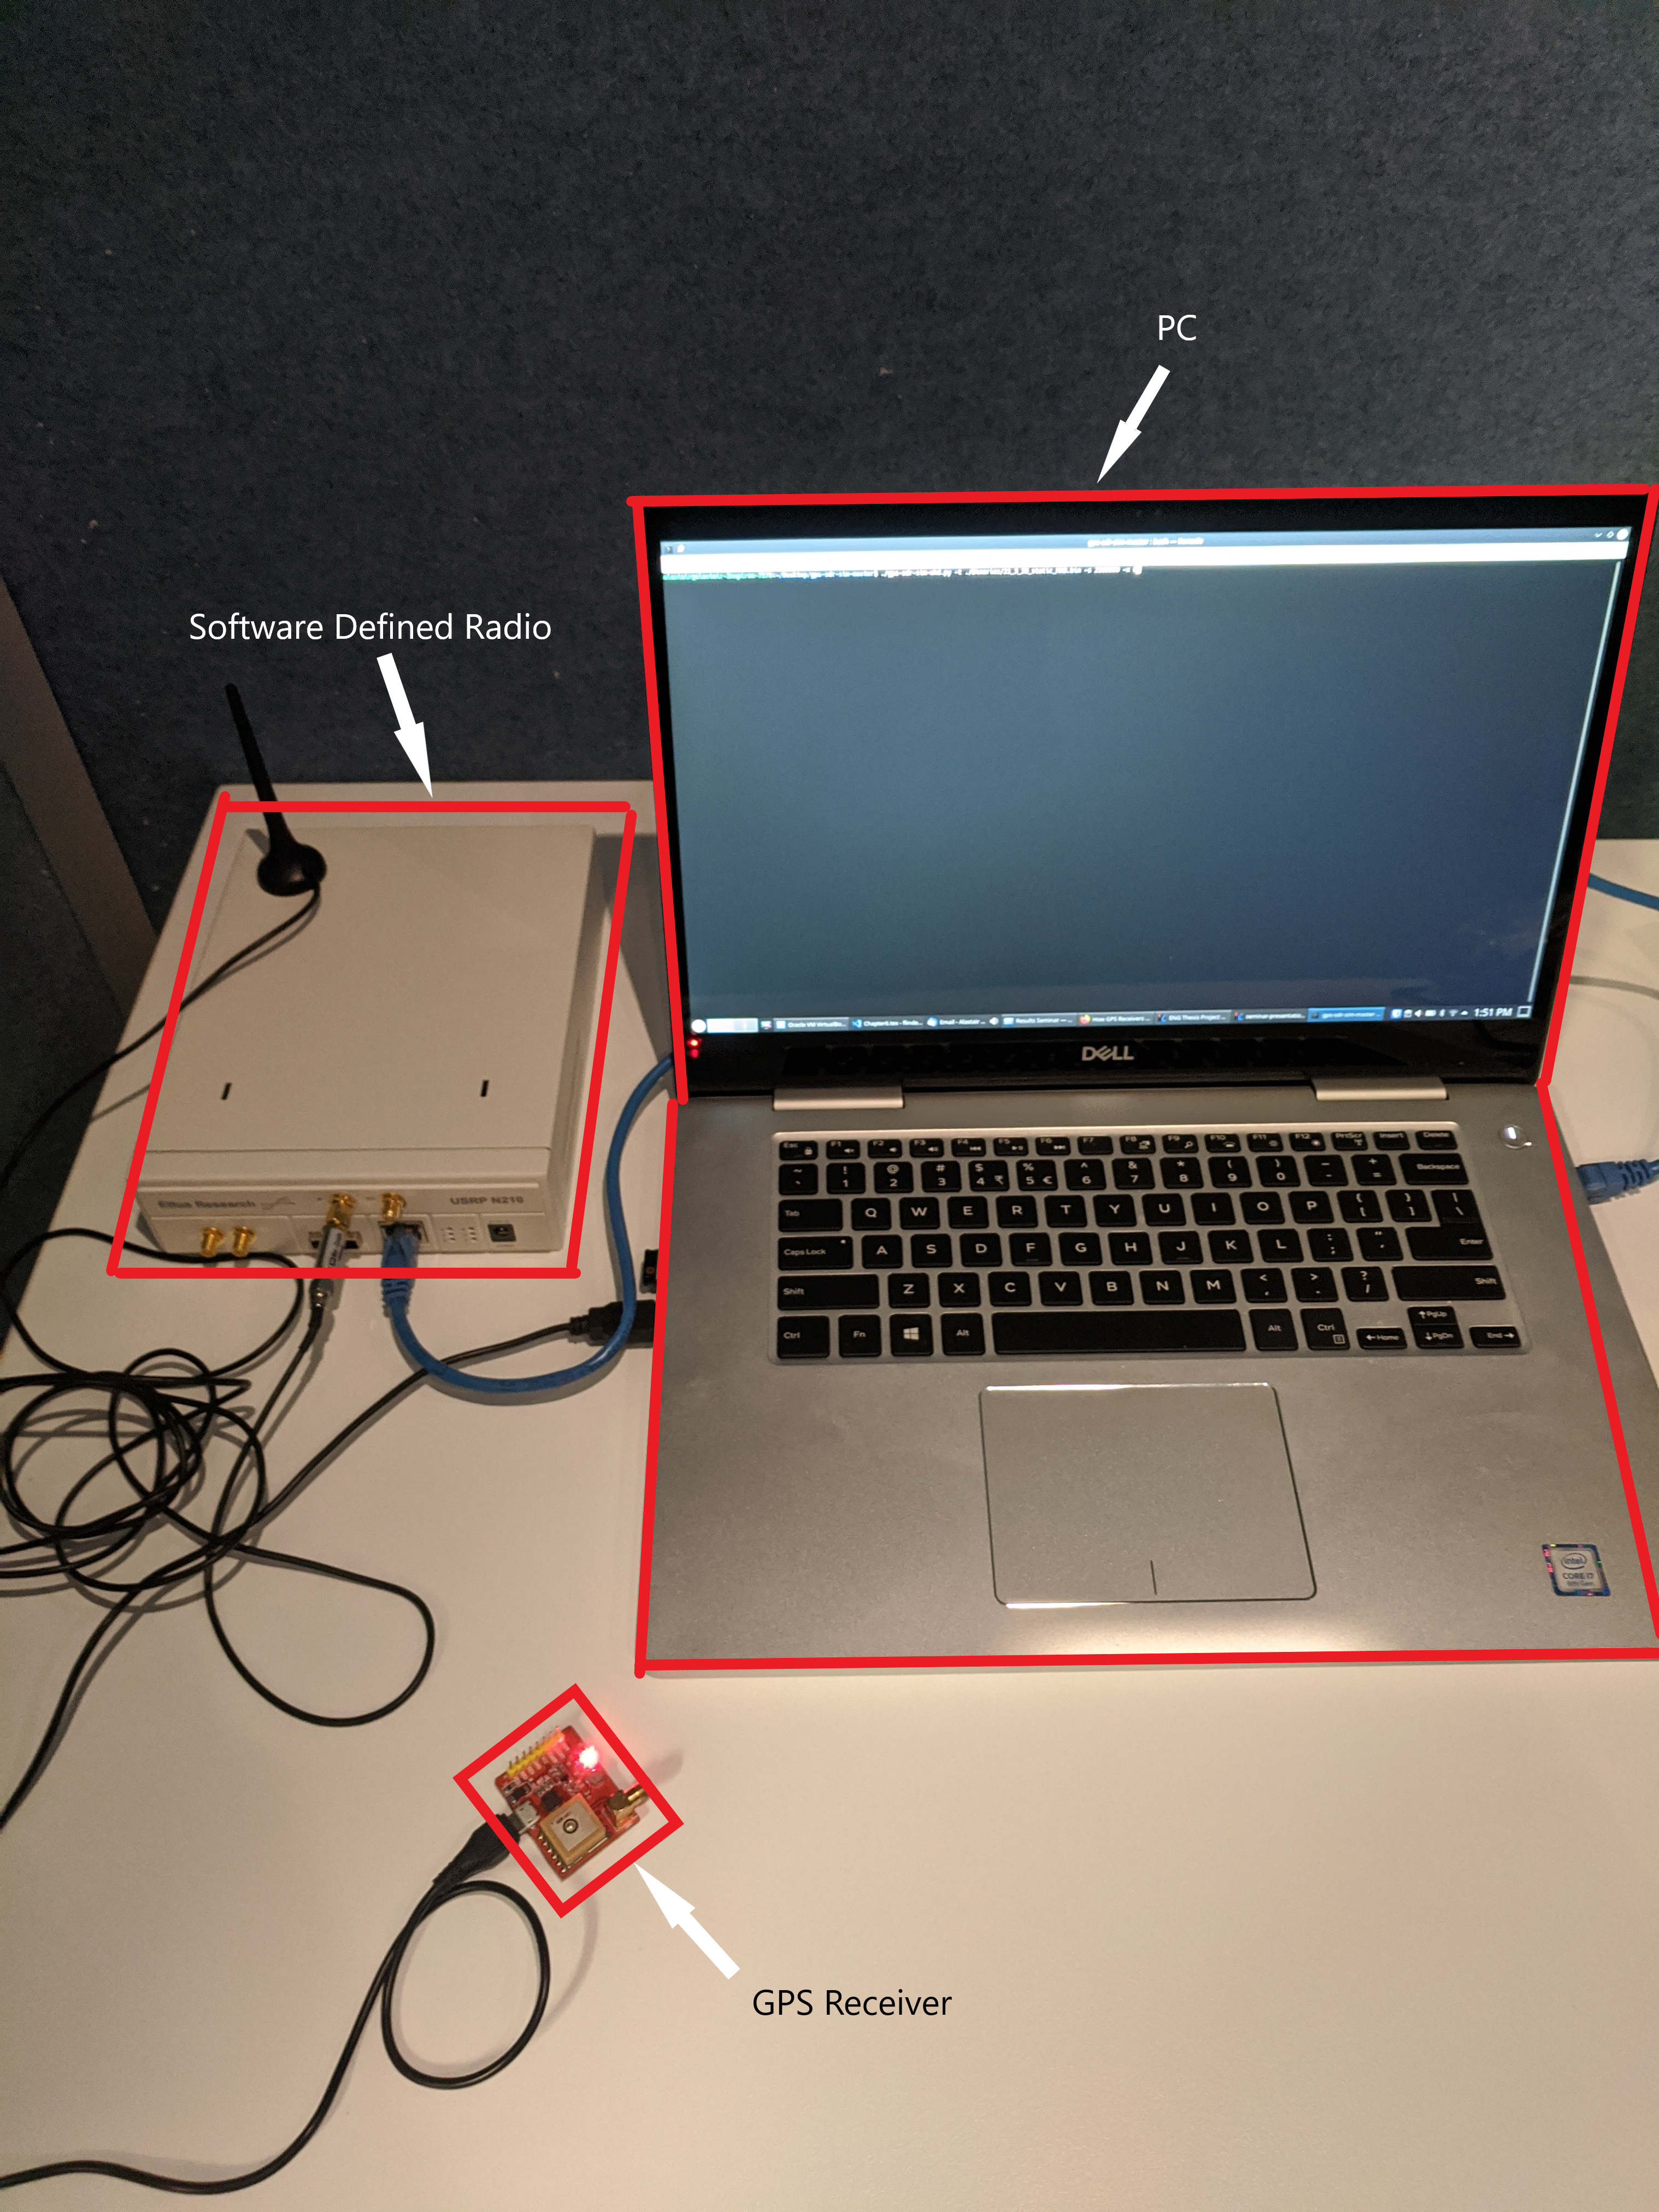
\includegraphics[width=13cm,keepaspectratio]{Figures/Setup/overview_labelled.png}
        \caption{Hardware setup for testing spoofing transmission within Faraday cage}
    \label{fig:HardwareSetup}
    \end{centering}
\end{figure}

\subsection{SDR Setup for GNSS Reception}
Reception of GNSS signals is a complicated process which involves synchronising time values and solving simultaneous equations for position, therefore instead of
developing the software from scratch it was decided that
the open-source program GNSS-SDR would be used to perform all of these functions. This software has been built over a number of years and is able to receive different GNSS
signals and translate them into position \cite{RN16}.

The hardware setup for GPS signal reception was different. Since the signal strength of a GNSS transmission is so low when it reaches the earths surface ($\approx -160dBm$) an active
antenna is typically required for best performance, especially if there is no clear view of the sky or if there are many buildings that add multipath signals into
consideration. In order to use an active antenna with the SBX daughtercard a device called a Bias-T was required. The active antenna typically requires 3.3-5V DC to
power the LNA (low noise amplifier) and any filters. This is done by injecting the voltage as an offset onto the antenna cable, where it is filtered out before the ADC
(analog to digital converter) of
the RF front end. This is not available internally to the SDR, thus is handled by the bias-T externally. A schematic of the bias-t setup is shown in figure \ref{fig:biasT}.

\begin{figure}[h]
    \begin{centering}
        \includegraphics[width=12cm,keepaspectratio]{Figures/biasT setup.png}
        \caption{Schematic of how the Bias-T was installed between the antenna and the USRP RX antenna port to allow for DC injection to the antenna and DC filtering to the SDR}
        \label{fig:biasT}
    \end{centering}
\end{figure}

\section{Software Setup}
The laptop was the interface between software and hardware. It was used to generate the binary files and then to control the SDR. The SDR would not operate without the
PC attached to the ethernet port.

The software used for this project was a combination of open source and custom software. 
The software was chosen while performing the literature review. There were examples \cite{RN4} \cite{RN28} of using open source programs
for the purpose of GPS spoofing. This was the best step forward since there were credible results with that software.

Custom software was created for the reporting and results of the experiments. 

\begin{itemize}
    \item GPS-SDR-sim
    \item GNURadio
    \item GNSS-SDR
    \item Python3
\end{itemize}

\section{Faraday Cage} \label{sec:FaraCage}
A Faraday cage was used for testing purposes for two main reasons. It will isolate the target device from existing legitimate GNSS signals and stop any transmitted
radiation from propagating into the local environment. Isolation from receiving legitimate signals is important since a receiver that is tracking a satellite already is
harder to jam or spoof than one that is not. More important is ensuring that the radiation does not enter the environment since transmitting any signals on the frequency
band for GNSS systems is illegal in Australia. 

Since the received signal strength from a GNSS satellite is so low ($\approx -150dBm$) any signal that is transmitted from Earth's surface will be able overpower these
signals for up to 85km, assuming an omnidirectional antenna, as shown in equation \ref{eq:propogationCalc}. This calculation was performed with the assumed maximum
transmission power of the SDR of $15 dBm$ coupled with a $30dB$ attenuator and transmitting on the L1 GPS band. In practise the effective range will be much less due to
attenuation due to objects between transmitter and receiver, but this calculation shows that performing the experiments within a controlled environment was required.
\begin{equation}    
    \begin{split} \label{eq:propogationCalc}
        Att_{dB} &= 10 \log_{10}\left(\frac{c}{4\pi df}\right)^2 \\
        d = \frac{c}{4\pi 10^{\left(\frac{Att_{dB}}{20}\right)}f} &= \frac{3\times10^8}{4\pi 10^{-6.75}1.57542\times 10^9} \approx 85km
    \end{split}
\end{equation}

%----------------------------------------------------------------------------------------
%	SECTION 3
%----------------------------------------------------------------------------------------

\section{Testing Workflow}

Some preliminary testing was done with different software setups to see which would be the best for reproducing spoofing results. A combination of meaconing and signal
generating techniques were investigated. Initially meaconing was chosen as the best way to perform an attack, therefore an attempt was made to record real time GPS signals
and store them for later transmission. Initial testing using a passive log periodic antenna resulted in no data being properly captured. Since a log-periodic antenna was
used there was a mismatch in the polarisation of the wave. The transmitted GPS signal is polarised as RHCP, whereas by its nature log-periodic antennas are linearly
polarised. This polarity difference equated to a $3dB$ attenuation of the signal. This coupled with the lack of signal gain from the passive antenna and the directional nature of the antenna
meant that the data within the signal was unrecoverable and an active antenna should be used. Unfortunately, none of the daughtercards on hand were able to feed an active
antenna. A bias-tee was used in order to feed the antenna with the $5V$ required for its operation while filtering out the DC to feed into the SDR. To interface with the
bias-tee a USB cable was cut and used to connect to a perf board with a soldered SMA connector. Unfortunately this was unsuccessful. The GNSS-SDR program was unable to
find or lock onto any of the GPS satellites at any time. It was found that another open-source program, GPS-SDR-sim, could be used to create binary files that replicate
the received signals from the satellites. 
\\Through experimentation a successful workflow was created, as shown in figure \ref{fig:Flowchart}.

\begin{figure}[H]
    \begin{center}
        \begin{tikzpicture}
            \begin{centering}
                \node[stepNode][draw, text width=3cm,minimum height=1.5cm](block1){Choose \\ Coordinates};
                \node[stepNode][draw, below=of block1, text width=3cm,minimum height=1.5cm](block2){Generate \\NMEA file};
                \node[stepNode][draw, below=of block2, text width=3cm,minimum height=1.5cm](block3){Download ephemeris};
                \node[stepNode][draw, below=of block3, text width=3cm,minimum height=1.5cm](block4){Compile \\Signal Binary File};
                \node[stepNode][draw, below=of block4, text width=3cm,minimum height=1.5cm](block5){Transmit Signal};
                \node[stepNode][draw, below=of block5, text width=3cm,minimum height=1.5cm](block6){Log GPS Data};
                \node[stepNode][draw, below=of block6, text width=3cm,minimum height=1.5cm](block7){Generate Graphs};
            \end{centering}

                \draw[-latex] (block1) edge (block2) (block2) edge (block3) (block3) edge (block4) (block4) edge (block5) (block5) edge (block6) (block6) edge (block7);
        \end{tikzpicture}
    \end{center}
    \caption{Flowchart of performing experimentation. Each of the nodes will be expanded upon in the sections below} \label{fig:Flowchart}
\end{figure}

\subsection{Choose Coordinates} \label{subsec:coordinate}
Regardless of whether a static or dynamic spoofing attack is desired, the best way to choose the coordinates was through the use of SatGen3. There was an alternative for
static scenarios which did remove the need for installing SatGen3. This alternative was through the use of GPS-SDR-sim itself. It has an attribute that allows for
inputting either latitude longitude or ECEF coordinates. So while this does save one step, it still requires using a map software to find the desired coordinates, which
is considerably simplified using SatGen3. To compile dynamic situations a GGA NMEA stream is always required. Considering for this project there was a desire to have both static and dynamic spoofing it made sense
to maintain a more consistent workflow.

Figure \ref{fig:StaticCoordinate} shows the searching and selecting of a coordinate for use in a static spoof attack within the SatGen3 application. The
SatGen3 program has access to the google maps API and allows for searching. This makes finding the desired location for spoofing attack easy. 
Figure \ref{fig:DynamicCoordinate} shows mapping out of a path within SatGen3 in order to generate a dynamic spoof attack.

\begin{figure}
    \begin{centering}
        \includegraphics[width=12cm,keepaspectratio]{Figures/static coordinates setup.png}
        \caption{Using google maps within SatGen3 to choose a static coordinate to be used as desired spoof location}
    \label{fig:StaticCoordinate}
    \end{centering}
\end{figure}

\begin{figure}[ht]
    \begin{centering}
        \includegraphics[width=12cm,keepaspectratio]{Figures/dynamic coordinates setup.png}
        \caption{Using google maps within SatGen3 to choose a set of coordinates to be used as desired spoof path for a dynamic spoof attack}
    \label{fig:DynamicCoordinate}
    \end{centering}
\end{figure}

\subsection{Generate NMEA File} \label{subsec:NMEAFile}
The coordinate and NMEA file creation step is essentially the same step within the SatGen3 software package. Once the coordinate or path was chosen, it was a matter of
choosing to save the output as a text file. An example of this is shown in Figure \ref{fig:StaticCoordinateNMEA}. In order to keep track of the source NMEA files and the
results files the following naming scheme was employed:
\\
\begin{verbatim}
    YY_MM_DD_<static/dynamic>_LOCATION.nmea
    YY_MM_DD_<static/dynamic>_LOCATION.bin
    YY_MM_DD_<static/dynamic>_LOCATION.txt
\end{verbatim}

Where .nmea file was the source file, the .bin file was the signal binary file and the .txt file was the log file produced from the GPS receiver.

When generating a dynamic file there is an option to set the amount of "stationary" time. This will put a buffer of unmoving coordinates for a set amount of time. This
was used to allow the spoofing victim time to lock onto the spoofed signal before the simulated movement began.

To generate the binary bit stream for use with an SDR RF front end a GGA NMEA data stream was created using the SatGen3 software package. This NMEA stream was used to make
the binary file using the GPS-SDR-sim command line interface program. SatGen3 replaces the need for capturing the raw GNSS signals or GGA sentence stream thus increasing
the flexibility of scenarios that can be tested. Although there is no guarantee that the simulated stream of information is going to be correct. Thus a capture replay
attack should still be considered as more reliable.

\begin{figure}[!ht]
    \begin{centering}
        \includegraphics[width=12cm,keepaspectratio]{Figures/2021_03_30_static_MAB_setup.png}
        \caption{Using static coordinate to generate NMEA file}
    \label{fig:StaticCoordinateNMEA}
    \end{centering}
\end{figure}

\subsection{Download Ephemeris}
From the NASA website, hourly versions of the GPS constellation ephemeris, in the form of a RINEX file, are available. These are compiled into a daily file. These daily
files are available all the way from 1992. An account is required to access these files, but there are sample programs provided for retrieving
the files programatically using different methods. A script was generated that was able to get the latest version from the website using Python. The full version of this
script is shown in Appendix \ref{sec:EphemerisCode}. There were initially some
issues with getting the script to connect to the remote server to gain access to the files. It was found that there was a bug on Linux with a certain version of openssl.
A newer version was manually installed and this solved the issue.

The downloaded file was a compressed version of the text file, and thus it was required to be uncompressed using the tar program.

\subsection{Compile Signal Binary File}
GPS-SDR-sim compiles the signals into a 16bit data format where the first 8bits represents the in-phase data and the next 8 bits represents the Quadrature data information.
The minimum requirements to compile a binary file using GPS-SDR-SIM was a source coordinate in either ECEF or latitude/longitude format and the ephemeris for the desired date and time that the spoofer
will transmit. This did not need to match the date and time that the signal was being transmitted on. If the attack was to be a dynamic spoofing attack then it was
required that there be a "user motion file" or GGA sentence stream. This stream was required to be 10Hz. It was decided that even for static scenarios a GGA stream would
be used. This simplified the workflow overall. Using this method meant that the program was able to calculate the duration of the transmission itself. The output was
altered in order to conform with the naming convention stated in Section \ref{subsec:NMEAFile}. The sampling rate was also modified to be 2.5Msps instead of the default
2.6Msps.
When compiling some of the dynamic spoofing scenarios the maximum size was reached. This is a limit that is hard coded when the GPS-SDR-sim program is compiled on the host
machine. Therefore, the program was cleanly recompiled in with the command to increase the maximum size of output file.

Using this information, the place, time and ephemeris the program is able to calculate which of the satellites will be in view and what their expected pseudoranges would
be. This is shown in Figure \ref{fig:sdrsimexample}.
The signal modulation is applied within the compilation of the file, simplifying the process of transmitting the file. 

\begin{figure}[!ht]
    \begin{centering}
        \includegraphics[width=14cm,keepaspectratio]{Figures/gps-sdr-sim options.png}
        \caption{Options available for compiling spoofed GPS signal using the GPS-SDR-SIM program}
    \label{fig:sdrsimoptions}
    \end{centering}
\end{figure}

\begin{figure}[!ht]
    \begin{centering}
        \includegraphics[width=14cm,keepaspectratio]{Figures/gps-sdr-sim running.png}
        \caption{Example of running GPS-SDR-sim with required arguments to generate dynamic spoof around the Tonsley MAB}
    \label{fig:sdrsimexample}
    \end{centering}
\end{figure}

\subsection{Transmit Signal}
Once the signal has been compiled into a binary file it is sent to the USRP SDR via GNURadio. GNURadio has an SDK that allows for text based programming. A script that was
capable of connecting to USRP devices automatically through the UHD (USRP Hardware Driver) daemon was distributed with the GPS-SDR-sim program. This was used to simplify the development
process. 

This was a simple program that connected the source file to the SDR via some simple blocks as shown in Figure \ref{fig:GNURadioSpoof}. The file is read 16bits at a time
into the "IShort to Complex" block. This converts the interleaved I/Q data into a complex file type which is then passed to the SDR via an amplifier block.

\begin{figure}[!ht]
    \begin{centering}
        \makebox[\textwidth][c]{\includegraphics[width=1.12\textwidth]{Figures/GNURadio_Spoofer.png}}%
        % \includegraphics[width=14cm,keepaspectratio]{Figures/GNURadio_Spoofer.png}
        \caption{GNURadio flowchart for transmitting binary files with USRP}
    \label{fig:GNURadioSpoof}
    \end{centering}
\end{figure}

An important part of the transmission was that it needed to be performed within a Faraday cage for legal purposes. This was discussed in section \ref{sec:FaraCage}.

\subsection{Log GPS Data}
To log the transmitted GPS signals from the SDR a COTS receiver and a smartphone were set up. The COTS receiver has a USB interface that outputs a stream of NMEA
sentences at a 1Hz frequency. This can be modified to 5Hz, but this was not required for these experiments. Using a script the USB port was opened and logged to a text
file, see Appendix \ref{sec:GPSConnect}. The log file was passed as an argument and could be stored wherever it was needed. Each time a spoof attempt was made, the GPS
receiver was powered off to ensure there was not lock when starting the experiment. This ensured results were as consistent as possible.

When using a smartphone, Android was required for logging since the OS allows access to the raw properties of the received signal. These properties include, as of Android
7.0, Position, velocity, C/No, satellite/constellation, pseudorange, navigation messages, accumulated delta range and hardware clock \cite{RN39}.
There is also an intuitive application
"GNSS Logger" that allows for comprehensive visualisation of current GNSS tracking as well as the ability to log data. This data was logged to a text file using a non
standard layout, but there was an option to log the NMEA sentences as well.  

\subsection{Generate Graphs}
Once there was a log file, graphs were generated to visualise the various parameters of the location resolution as interpreted by the receiver. 
The generation of the graphs that make up the results section was done in python and was based upon the NMEA sentences logged from the receivers. GPS receivers have the
ability to check the validity of signals they receive. When they are able to resolve a location the value of one of the fields within the RMC sentence is changed to
reflect this. The number of sentences before initial lock were counted. This was
used to determine the time to first fix of each test since it was known that the GPS receiver would output at 1Hz. Alterations would need to be made if the receiver was
outputting at a higher frequency. As such this should not be considered accurate and viewed as an estimate only.

The carrier to noise ratio graphs were generated directly from the output of the GSV sentences. The SVID and associated $\frac{C}{N_0}$ ratios were stored as the value in
a key value pair. The key was a timestamp used to ensure each sentence was represented.\\
The latitude and longitude were retrieved from the GGA sentences.

Using the NMEA stream created in section \ref{subsec:NMEAFile} a desired plot was put on both the static and dynamic graphs. For the static graphs this reference was also
used as the origin when calculating the error of the calculated location.

The error was calculated by finding the difference in latitude and longitude from the desired origin point and converting the $\Delta Lat$ and $\Delta Long$ into meters.
This assumes that the distances being dealt with are so small that they are essentially flat. Thus the equations can be simplified to remove any angles.

The earth is not perfectly spherical therefore when converting latitude and longitude into $x$ and $y$ coordinates in meters the average of the polar plane and equatorial
planes were taken, as shown in equation \ref{eq:EarthCircumference}. The $\Delta x$ and $\Delta y$ values from Equation \ref{eq:deltaX} and \ref{eq:deltaY} represent
the error of the coordinate in the $x$ and $y$ direction respectively. \\
When finding the total error value the law of Haversines was used, see equation \ref{eq:Haversine}, where $\phi_i$ and $\lambda_i$ are the latitude and longitude of the
$i^{th}$ coordinate respectively, and $r$ is the radius if the sphere in question. For this use case it is the average radius of the Earth.  

\begin{equation} 
    \begin{split} \label{eq:EarthCircumference}
        C_{Polar} = 40007.863 km \\ 
        C_{Equatorial} = 40075.017 km
    \end{split}
\end{equation}

\begin{equation} \label{eq:deltaX}
    \Delta x = \Delta Lat \times \frac{C_{Polar}}{\frac{2}{180}} \times 1000 m
\end{equation}

\begin{equation} \label{eq:deltaY}
    \Delta y = \Delta Long \times \frac{C_{Equatorial}}{\frac{4}{90}} \times 1000 m
\end{equation}

\begin{equation} \label{eq:Haversine}
    d = 2r \arcsin\left(\sqrt{\sin^2\left(\frac{\phi_2 - \phi_1}{2}\right) + \cos\left(\phi_1\right)\cos\left(\phi_2\right)\sin^2\left(\frac{\lambda_2 - \lambda_1}{2}\right)}\right)
\end{equation}
 
Below (Listing \ref{list:pythonHaversines}) is the implementation of the law of Haversines in python used for the calculation of distance between two latitude and longitude points. The output of the function was stored
into an array and used to graph the total error over time for static spoofing attacks.

% \begin{verbatim}
%     def latlon2m(lat1, long1, lat2, long2):
%         r = 6371000  
%         dLat = radians(lat2) - radians(lat1)
%         dLong = radians(long2) - radians(long1)
%         a = math.sin(dLat/2) * math.sin(dLat/2) + 
%             math.cos(radians(lat1)) * math.cos(radians(lat2)) *
%             math.sin(dLong/2) * math.sin(dLong/2)
%         d = 2*r*math.asin(math.sqrt(a))
%         return d
% \end{verbatim}

\begin{lstinputlisting}[language=Python, label=list:pythonHaversines, caption=Python implementation of the law of Haversines used to calculate the distance between two points on a sphere, firstline=23, lastline=29]{NMEAParse.py}
\end{lstinputlisting}

There is a PC companion application for the GNSS Logger app that allows for comprehensive
graphing and reports to be generated for a particular log file.


\section{Experiments}
\subsection{Static Spoofing}
Within this thesis static spoofing is defined as producing a signal that produces a calculated location that does not change over time. While in practise there was some
minor movement caused by the uncertainty in trilateration and system errors, this change in position was typically minor and within the range of error of GPS positioning.
Using the SatGen3 software a location was chosen as the spoof location. After setting the desired time and date of spoofing the scenario was created and saved as a text file. 

\subsection{Dynamic Spoofing}
Dynamic spoofing refers to the production of a signal that when used to calculate position, will be shown to change over time. The path traced by the receiver will be
set at the time of production of the binary file, but there will be perceived motion from the GPS receiver.

\subsection{Real-Time Spoofing}
Due to time constraints a real-time algorithm was not produced as part of this project. However, utilising the open source projects that have been used to complete this
thesis, it would be probable to create a real time spoofing device that would be able to react to the positional changes of the receiver instead of following a
pre-determined path when generating the binary file. The signals generation algorithm could be ported to a GNURadio block in C++ to allow for easy access to real-time GPS
signal spoofing. If an SDR is a full duplex radio, such is the case for the USRP N210, then one port can be receiving the real GNSS signal and the other can be
transmitting the spoofed signal. Care would need to be taken in the set up of this arrangement since any transmitted signal would also be picked up by the receiving
antenna. Therefore a directional transmitting antenna and physical distance should be employed to allow for legitimate GNSS signals to reach the receiver port.  
% Chapter Template

\chapter{Results} % Main chapter title

\label{Chapter5} % Change X to a consecutive number; for referencing this chapter elsewhere, use \ref{ChapterX}

This section covers the results of the GNSS reception and GPS transmission experiments. Section \ref{sec:Res_GNSSReception} covers the attempts at receiving authentic GNSS
signals and accurately calculating a location. Section \ref{sec:Res_GPSTransmission} will cover the attempts and results of performing spoofing attacks on GPS receivers.
%----------------------------------------------------------------------------------------
%	SECTION 1
%----------------------------------------------------------------------------------------

\section{GNSS Reception} \label{sec:Res_GNSSReception}
Before testing the GPS transmission performance of the SDR, reception was tested, with less success. Three antenna setups were chosen each failing to lock and track the
satellites. A log linear, an omnidirectional and an active patch antenna were all used. The active antenna should have given best results since it includes amplifiers and
filters within the antenna module itself. The failure could be to do with the bias-t used to inject the 5V DC into the antenna, however testing with a multi-meter showed
that there was 5V on the RF+DC port of the Tee.

%----------------------------------------------------------------------------------------
%	SECTION 2
%----------------------------------------------------------------------------------------

\section{GPS Transmission} \label{sec:Res_GPSTransmission}
Experimentation was performed at the Tonsley campus of Flinders University, which has coordinates of $-35.007650, 138.572030$. At first it was decided to use the
centre of the Adelaide CBD as the coordinates for spoofing, that is $-34.5571732282, 138.3599516878$. Therefore it would be considered successful if the GPS receiver was to show
that the current location was in the CBD. This was extended to include other locations, Davis Station in Antarctica and the MAB at Flinders University Tonsley Campus with
coordinates of $-68.5762449235, 77.9696166515$ and $-35.00792163316667, 138.5715065625$ respectively.

Dynamic spoofing attacks were set to the road surrounding the MAB and around the CBD of Adelaide. All spoof attack dates were set to the same date, which was chosen to be
the 30th March 2021. This was arbitrary and only chosen since this was when official testing began.

\subsection{Meaconing Attack}
Since the GPS reception failed with the SDR, there was no way of performing a meaconing attack. Therefore, the only viable attack strategy was to generate a binary file
of the intended location. It would be ideal to perform this kind of attack in the future since this is the only basic attack type that can be used on the encrypted
military band.

\subsection{Spoofing Attack}
Once the workflow and hardware setup for the SDR was properly configured it was found that a smartphone was able to be spoofed.
When attempting to spoof devices in the wild, the Pixel XL smartphone was susceptible to attack while more modern smartphones that were tested were not susceptible. These
included the iPhone 12 Pro, Samsung Galaxy S10 and Google Pixel 3XL. The spoofing setup was not able to fool any of these devices. This could be down to software based
anti-spoofing algorithms that have been implemented including the usage of multiple constellations for position resolution.

\subsection{Static Spoofing}
\subsubsection{Tonsley MAB}
The grassed area outside of the Flinders University Tonsley campus was chosen as one of the points to spoof to. As mentioend above the desired coordinates that the receiver were
$-35.00792163316667, 138.5715065625$.

From Figure \ref{fig:MABStaticPosition} it can be seen that there are negative numbers, this is arbitrary and was included in order to give perspective as to which direction
the received position was wrong.

In this example the time to first fix was calculated as being 37 seconds. This is quite good for a cold start situation. During experimentation the time to first fix has
been variable between 30 seconds and 180 seconds. A trend has been the quicker the fix the better the overall accuracy of the spoofed location.

\begin{figure}[!h]
    \begin{centering}
        \includegraphics[width=14cm,keepaspectratio]{Figures/2021_3_30_static_MAB Carrier noise ratio.png}
        \caption{Carrier to noise ratio from unique SVIDs as broadcast by SDR and received by GPS receiver at MAB in Tonsley on 30th March 2021. Each SVID has been given a unique colour.}
        \label{fig:MABStaticCNo}
    \end{centering}
\end{figure}

\begin{figure}[!h]
    \begin{centering}
        \includegraphics[width=14cm,keepaspectratio]{Figures/2021_3_30_static_MAB Lat long position.png}
        \caption{Trace of latitude and longitude over time as interpreted from the GPS receiver with expected location noted with red dot}
        \label{fig:MABStaticCoord}
    \end{centering}
\end{figure}

\begin{figure}[!h]
    \begin{centering}
        \includegraphics[width=14cm,keepaspectratio]{Figures/2021_3_30_static_MAB Position from origin.png}
        \caption{Graph of recorded position with respect to the intended spoofed location}
        \label{fig:MABStaticPosition}
    \end{centering}
\end{figure}

\begin{figure}[!h]
    \begin{centering}
        \includegraphics[width=14cm,keepaspectratio]{Figures/2021_3_30_static_MAB error over time.png}
        \caption{Error between calculated location and expected location over time}
        \label{fig:MABStaticError}
    \end{centering}
\end{figure}

\begin{figure}[!h]
    \begin{centering}
        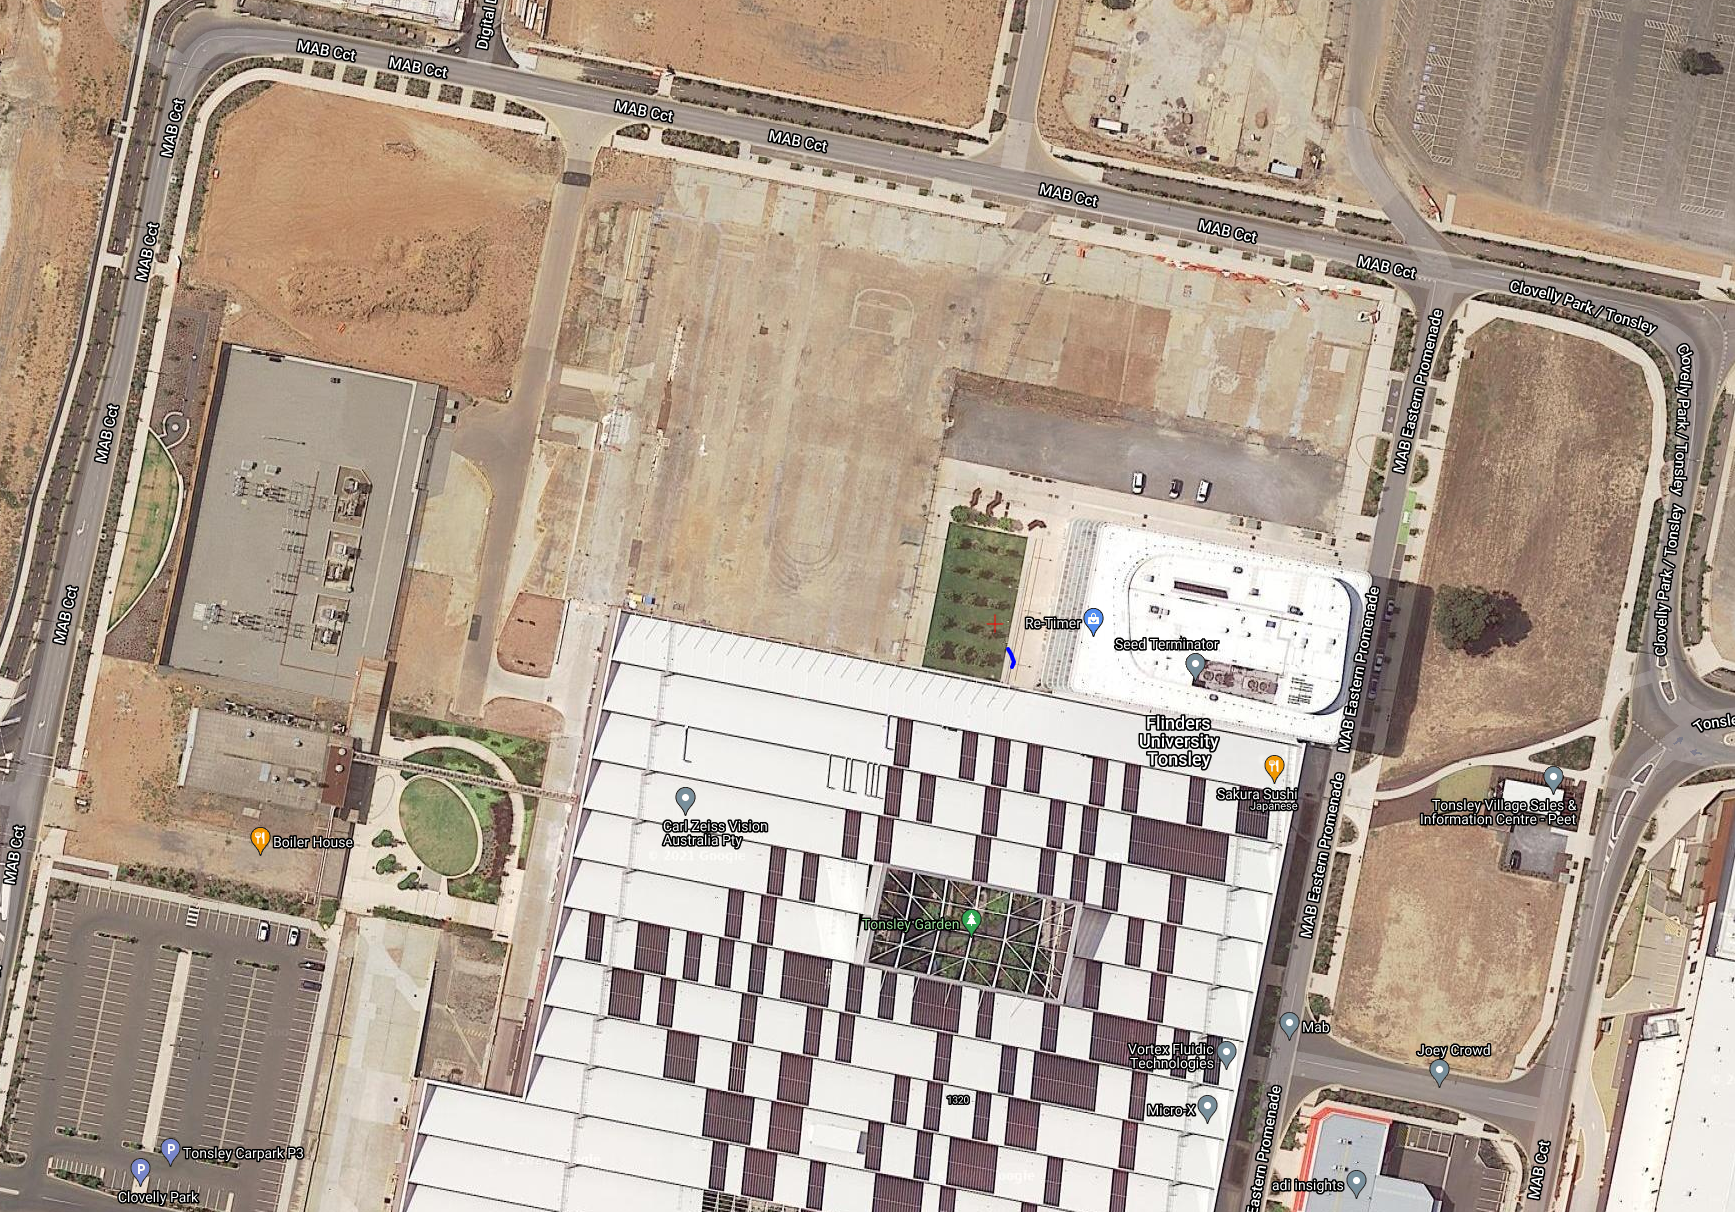
\includegraphics[width=14cm,keepaspectratio]{Figures/2021_3_30_static_MAB_Satellite.PNG}
        \caption{Satellite image with expected GPS position shown with red cross and recorded position shown with blue line}
        \label{fig:MABSatelliteImage}
    \end{centering}
\end{figure}

\subsubsection{Antarctica}
Davis station in Antarctica was chosen as a location for spoofing. As mentioned above the coordinates for this location was $-68.5762449235, 77.9696166515$. The COTS
receiver was used as a spoof victim and it was successfully spoofed. Figure \ref{fig:antarcticaStaticCNo} shows the carrier to noise graph over the spoof attack. There is
a consistent value of $\approx 50 dBHz$ plus signals that are consistently at $\approx 40 dBHz$. Time to first fix was shown to be approximately 60 seconds, this is the
lower end of the fix times from experiments for cold starts. It can be see that there is consistent signals for the first 50 seconds. For the time pereiod between 70 and
200 seconds there was more volatile signal quality. Figure \ref{fig:antarcticaStaticError} shows that there was a high, but consistent level of error between first fix
and 140 seconds. After this there was a spike, which is associated with a drop of lock, and the high error remained until the end of the test. This high error is evident
when viewing the raw position in Figure \ref{fig:antarcticaStaticCoord} and with respect to the desired location, Figure \ref{fig:antarcticaStaticPosition}. Figure \ref{fig:antarcticaSatelliteImage} shows this error
in position in more context placed over a satellite image.
The inaccuracy is higher than was expected from this experiment.  

\begin{figure}[!h]
    \begin{centering}
        \includegraphics[width=14cm,keepaspectratio]{Figures/2021_3_30_static_antarctica Carrier noise ratio.png}
        \caption{Carrier to noise ratio from unique SVIDs as broadcast by SDR and received by GPS receiver at Davis Station in Antarctica on 30th March 2021. Each SVID has been given a unique colour.}
        \label{fig:antarcticaStaticCNo}
    \end{centering}
\end{figure}

\begin{figure}[!h]
    \begin{centering}
        \includegraphics[width=14cm,keepaspectratio]{Figures/2021_3_30_static_antarctica Lat long position.png}
        \caption{Trace of latitude and longitude over time as interpreted from the GPS receiver with expected location noted with red dot}
        \label{fig:antarcticaStaticCoord}
    \end{centering}
\end{figure}

\begin{figure}[!h]
    \begin{centering}
        \includegraphics[width=14cm,keepaspectratio]{Figures/2021_3_30_static_antarctica Position from origin.png}
        \caption{Graph of recorded position with respect to the intended spoofed location}
        \label{fig:antarcticaStaticPosition}
    \end{centering}
\end{figure}

\begin{figure}[!h]
    \begin{centering}
        \includegraphics[width=14cm,keepaspectratio]{Figures/2021_3_30_static_antarctica error over time.png}
        \caption{Error between calculated location and expected location over time}
        \label{fig:antarcticaStaticError}
    \end{centering}
\end{figure}

\begin{figure}[!h]
    \begin{centering}
        \includegraphics[width=14cm,keepaspectratio]{Figures/2021_3_30_static_antarctica_Satellite.PNG}
        \caption{Satellite image with expected GPS position shown with red cross and recorded position shown with blue line}
        \label{fig:antarcticaSatelliteImage}
    \end{centering}
\end{figure}

\subsection{Dynamic Spoofing}

\subsubsection{Tonsley MAB}
The time to first fix was shown to be approximately 49 seconds.


\begin{figure}[h]
    \begin{centering}
        \includegraphics[width=14cm,keepaspectratio]{Figures/2021_3_30_dynamic_MAB Carrier noise ratio.png}
        \caption{Carrier to noise ratio from unique SVIDs as broadcast by SDR and received by GPS receiver at MAB in Tonsley on 30th March 2021. Each SVID has been given a unique colour.}
        \label{fig:MABdynamicCNo}
    \end{centering}
\end{figure}

\begin{figure}[h]
    \begin{centering}
        \includegraphics[width=14cm,keepaspectratio]{Figures/2021_3_30_dynamic_MAB Lat long position.png}
        \caption{Trace of latitude and longitude over time as interpreted from the GPS receiver with expected location noted with red dot}
        \label{fig:MABdynamicCoord}
    \end{centering}
\end{figure}

\begin{figure}[h]
    \begin{centering}
        \includegraphics[width=14cm,keepaspectratio]{Figures/2021_3_30_dynamic_MAB Position from origin.png}
        \caption{Graph of recorded position with respect to the intended spoofed location}
        \label{fig:MABdynamicPosition}
    \end{centering}
\end{figure}

\begin{figure}[h]
    \begin{centering}
        \includegraphics[width=14cm,keepaspectratio]{Figures/2021_3_30_dynamic_MAB_Satellite.PNG}
        \caption{Satellite image with expected GPS position shown with red cross and recorded position shown with blue line}
        \label{fig:MABdynamicSatelliteImage}
    \end{centering}
\end{figure}

\subsection{Issues Encountered}
The under run issue was more or less solved by increasing the buffer size to $40\times$ greater than the sampling size.
There was an issue towards the end of the project where there was considerable leakage of EM radiation into the Faraday cage that was causing the GPS receiver to produce
wildly inaccurate position (up to and over 500m error). This was much different to what had previously been recorded within the Faraday cage. This amount of error does
not constitute a successful spoof since the time to first lock was much greater than a real signal, or even spoofing attempts previously. 

During initial testing of the spoofing there was an inability to get the spoofer to correctly spoof the receiver. It was found that there is a requirement that the ratio
between the sampling frequency and clock frequency of the radio must be an integer value. Therefore when compiling the signal using GPS-SDR-sim the sampling frequency
value was required to be changed to 2.5Msps.  

Just after the testing phase of the project the smartphone that was being used for some of the logging and graphing was rendered unusable. While there was no data lost,
it was replaced with a newer model that experimentally was much harder to spoof than the previous model. This could be due to many factors including anti-spoofing
algorithms \cite{RN39}. It would be a fair assessment that the newer device is able to receive more GNSS signals including augmented systems as well as other signals such as Wi-Fi.
The connection to the Wi-Fi signal was such that notifications were coming up on the phone while performing the experiments.

There were a number of unterminated cables that were running from outside of the cage to inside. This was seen as being the cause of the issues that were being faced. The
suspect cables were removed or terminated and the results were more consistent with what was being achieved previously. Even with the new phone the GPS location was able
to be spoofed.

From sources \todo{insert source} it was found that the SVID and PRN are the same thing. 
A common result from spoofed attempts was to have GPS satellites with an SVID of over 100. GPS satellites have PRN codes from 1-63 and augmentation systems have PRNs from
64 to 158 \cite{RN67}. From the list of PRN codes \cite{RN67} it can be seen that the services that are being received are some kind of augmented system. \emph{This makes
me think that there might be a GBAS system or SBAS system nearby that is being received within the cage by stray wires etc.}

\section{Experimental Issues}
While performing experiments there were issues that were run into that were required to be overcome. Initially a Log Periodic antenna was used for transmission since its
frequency range was appropriate for use transmitting L1 band signals. After experiments failed to pick up any signals it was swapped for a omnidirectional antenna. This
was able to produce signals that were picked up by the GNSS Logger application. Observing the graphs of the carrier to noise figure showed that when there was an under run
issue the $\frac{C}{N_0}$ would drop to 0 and the GPS receiver in the phone would lose connection to the 'satellites'. This meant that no GPS lock was achievable.  

In an attempt to overcome the under run issue that was plaguing the experiments, a new PC was brought in with Ubuntu installed directly instead of via a VM. This resulted
in the radio working straight away. The under run issues resurfaced when trying to read the serial data from a COTS GPS receiver. This was less than ideal and required a
second computer to act as a datalogger.
 
% Chapter Template

\chapter{Discussion} % Main chapter title

\label{Chapter6} % Change X to a consecutive number; for referencing this chapter elsewhere, use \ref{ChapterX}
This section will discuss the results gathered from the previous section \ref{Chapter5}. Any braod findings or trends will be noted and explanations of why results are
the way they are.

%----------------------------------------------------------------------------------------
%	SECTION 1
%----------------------------------------------------------------------------------------

\section{Results}
Initially it was decided that the locations that would be spoofed would be locations that are not easily accessible as a means of proving the validity of the results.
This was made easier due to the ongoing pandemic. Although this idea was later changed to make it easier to compare with real signals if needed.

Using the developed workflow, it was simple to create and deploy spoofing attacks for any location and at any elapsed time within minutes. This includes static or dynamic
spoofing attacks. Not enough time was invested into the reception of GNSS signals and thus meaconing attacks were not performed. The GPS-SDR-sim program was able to
estimate and simulate the ionic effects. While it is clear that this method resulted in successful spoofing attacks, the hypothesis is that having a received signal that includes ionic delays
and other interference would make it easier to fool more complicated receivers. Further testing and investigations should be carried out to find the answer to this. 

The resutls from the static Antactica spoof attack, specifically the carrier to noise graphs show a high number of unique SVIDs. Based on the number of satellites in the
GPS constellation this must be an error. Although there was no explanation for the error since the resultant location was correct. One hypothesis was that the compilation
software added some incorrect data. Another is the prevelance of SBAS satellites. There was a known issue for some time with the Faraday cage where stray EM waves were
getting in. This would explain the connsistency in which SVID 193 appears. From \todo{ref} it can be seen that SVID 193 is a QZSS satellite.

SDRs are very sensitive to the processing pipeline of the computer that they are connected to. It is not uncommon to receive an under run error (where 'U' is printed to the
output) when transmitting a signal with high SPS (samples per second). This error is caused by the host computer not being able to feed the data to the radio quickly
enough.

This was solved by increasing the UDP buffer size manually to at least the sample rate, and over for better results. From limited experimentation this completely resolved the issue, and opened up
oppertunities to perform spoofing with low powered embedded devices like the Rasperry Pi single board computer.

\section{Future Work}
All of the tests that have been conducted for use in this thesis have either been generating a signal based off a predetermined location (coordinate) or a predetermined
path (group of connected coordinates). None of these options have a mechanism for position feedback. For example you cannot create a signal that has a linear offset from
the actual position using these methods. This is something that could be achieved through combination and modification of the exitisting open source projects used in this
thesis. This would allow for properly real-time gps spoofing, and could be extended further to have intelligent algorithms.

Current methods, as detailed in \ref{Chapter4}, requires downloading the Ephemeris for the date and time of the proposed spoofing attack. This makes real-time spoofing
attacks not possible since there is a delay between the current time and the associated ephemeris. A potential fix for this could be to perform some analysis on the
orbits of each satellite within the constellation over an arbitrary period of time to create a machine learning algorithm. This algorithm would be able to predict the
location of the satellites ahead of time, thus binaries could be compiled for future attacks, or could be used for real-time attacks without the need for downloading/
retrieving the ephemeris from legitimate sources.

Extended to work on anti-spoofing for PhD.

The logging program could be extended to provide real time feedback on position and signal quality. This would be acheived by implementating the serial connection wihtin
the Python code itself rather than relying on the logging function of screen.

The hardware used for this project was successfully used for spoofing attacks, howver, the software must be altered in order to achieve the accurate results that were
expected of the project. However ensuring software capabilities was out of the scope of this thesis.
% Chapter Template

\chapter{Chapter Title Here} % Main chapter title

\label{Chapter7} % Change X to a consecutive number; for referencing this chapter elsewhere, use \ref{ChapterX}

%----------------------------------------------------------------------------------------
%	SECTION 1
%----------------------------------------------------------------------------------------
% \include{Chapters/Chapter8}

%----------------------------------------------------------------------------------------
%	THESIS CONTENT - APPENDICES
%----------------------------------------------------------------------------------------

\appendix % Cue to tell LaTeX that the following "chapters" are Appendices

% Include the appendices of the thesis as separate files from the Appendices folder
% Uncomment the lines as you write the Appendices

% Appendix Template

\chapter{Project Code} % Main appendix title

\label{AppendixA} % Change X to a consecutive letter; for referencing this appendix elsewhere, use \ref{AppendixX}

\section{GPS Sentence Parsing and Graphing} \label{sec:NMEACode}
\textbf{Filename:} NMEA.py\\
\textbf{Description:} This code will take a NMEA file as input and calculate the time to first fix, then plot the carrier to noise ratio of every satellite that was
within view of the receiver, then plot the position given the output of the GPS receiver.

\begin{lstinputlisting}[language=Python, caption=Python code to parse the receiver NMEA sentence and produce graphs]{NMEAParse.py}
\end{lstinputlisting}

\section{GPS Ephemeris download script} \label{sec:EphemerisCode}
\textbf{Filename:} remote\textunderscore ephemeris\textunderscore utc.py\\
\textbf{Description:} This code will take the current time and and use that to request the latest ephemeris from the CDDIS portal.

\begin{lstinputlisting}[language=Python, caption=Python code to retreive the latest RINEX file from the CDDIS servers]{remote_ephemeris_utc.py}
\end{lstinputlisting}

\section{Connect to GPS Receiver} \label{sec:GPSConnect}
\textbf{Filename:} Connect\textunderscore receiver.sh\\
\textbf{Description:} Script that was used to set the permissions on the USB GPS receiver and then connect to the serial interface using the screen program. The script
would take 1 argument that was used to save the logfile.

\begin{lstlisting}[language=bash, caption=Bash script to connect to USB GPS receiver]
    #!/bin/bash

    filename=$1
    
    chmod 777 /dev/ttyUSB0
    screen -L -Logfile $filename /dev/ttyUSB0
   
\end{lstlisting}

% % Appendix Template

\chapter{GPS Receiver NMEA Sentence ouput} % Main appendix title

\label{AppendixB} % Change X to a consecutive letter; for referencing this appendix elsewhere, use \ref{AppendixX}

\section{Receiver Output}
Below is a snippet of the output from the GPS recevier unit used for testing.

\section{File used for generating binary}
Below is a snippet of the NMEA file that was used to generate the binary file. 
%\include{Appendices/AppendixC}

%----------------------------------------------------------------------------------------
%	BIBLIOGRAPHY
%----------------------------------------------------------------------------------------

\printbibliography
\end{document}  
